\documentclass[11pt]{article}

\usepackage[a4paper,margin=2.5cm]{geometry}
\usepackage{amsmath,amssymb,mathtools}
\usepackage{booktabs}
\usepackage{array,longtable}
\usepackage{needspace}
\usepackage{graphicx}
\usepackage{tikz}
\usetikzlibrary{arrows.meta,positioning,shapes.geometric}
\usepackage[hidelinks]{hyperref}
\usepackage{microtype}

\newcommand{\dd}{\mathrm d}
\newcommand{\Id}{\mathbf 1}
\newcommand{\eps}{\epsilon}
\newcolumntype{L}[1]{>{\raggedright\arraybackslash}p{#1}}

\title{FlintNDE: High-precision local-series transport for matrix differential equations}
\author{FlintNDE project}
\date{Draft of \today}

\begin{document}
\maketitle

\begin{abstract}
We present \texttt{FlintNDE}, a Python package built on FLINT for arbitrary-precision
numerical continuation of first-order matrix differential equations.  Its first core
function transports a boundary vector along a user path by local series, with automatic
ordinary/regular-singular dispatch, exact-first Frobenius and logarithm analysis, exact
Lee--Moser projector balances, certified exponential sectors, and an independent refinement chain.  Its
second core function repeats that solver at fixed
regulator values and reconstructs a semi-analytic Laurent series whose powers are analytic
and whose vector coefficients are high-precision numerical values.  This strategy avoids
carrying a symbolic regulator expansion through every relay point.  Exact
Gaussian-rational matrices provide an automatic finite and infinite singularity inventory;
general analytic evaluators use Cauchy--DFT coefficient extraction without symbolic
differentiation.  A higher-order pole initially certifies only that the supplied basis is
non-Fuchsian.  FlintNDE then applies exact projector balances built from the leading two
Laurent matrices, a strictly decoupled exponential-times-power--log ansatz, and, for a
rank-one irregular point with simple distinct leading roots, a start-only formal exponential
series with fixed-order five-term diagnostics.  Ramified or algebraic formal reductions,
Stokes matrices, and arbitrary Levelt--Turrittin problems remain fail closed.
\end{abstract}

\section{Introduction}

\subsection{Flat-space Feynman integrals}

Perturbative quantum-field-theory amplitudes are expressed through families of loop
integrals.  Integration-by-parts (IBP) identities reduce a family to finitely many master
integrals \cite{Chetyrkin:1981qh}; differentiating those masters with respect to a
kinematic, mass, or auxiliary parameter and reducing again gives a closed first-order
matrix differential equation \cite{Gehrmann:1999as}.  The remaining numerical problem is
to impose boundary data, cross singular regions, and evaluate the solution at physical
points.

Several public approaches expose complementary versions of this IBP--DE pipeline.
\texttt{DiffExp} joins one-dimensional local series along line segments in phase space
\cite{Hidding:2020ytt}.  AMFlow combines IBP reduction, auxiliary-mass differential
equations, systematic large-mass boundary data, and high-precision numerical transport to
compute general dimensionally regulated loop integrals
\cite{Liu:2022chg,Huang:2026rjb}.  FlintNDE adopts
one specific AMFlow component: it solves the complete problem at several fixed regulator
values and numerically reconstructs the Laurent coefficients.  In a long path with many
relay points, this avoids propagating an analytic regulator jet through every intermediate
matrix multiplication, which otherwise causes a rapid increase in algebraic complexity and
memory use.  The reconstruction remains numerical: it is checked by independent regulator
samples, not presented as an exact symbolic proof.

AmpRed provides another general IBP--DE route in the Feynman-parameter space
\cite{Chen:2024xwt}.  Its parameter integrals are organized in the Lee--Pomeransky (LP)
representation \cite{Lee:2013hzt}; parametric IBP relations construct the master system,
while asymptotic boundary data are organized with expansion by regions
\cite{Beneke:1997zp,Pak:2010pt}.  FlintNDE does not replace any reduction or region-analysis
frontend.  It consumes the resulting one-variable matrix system and certified boundary
data.

\subsection{de Sitter and cosmological integrals}

Massive fields during inflation leave characteristic non-Gaussian signals, motivating the
quasi-single-field and cosmological-collider programs
\cite{Chen:2009we,Chen:2009zp,Arkani-Hamed:2015bza}.  Here we mention only techniques that
directly construct IBP relations and differential equations.  The first two papers of the
dSIBP series formulate generalized IBP relations for time integrals and solve the resulting
systems, including multivariate hypergeometric and $\mathrm d\log$ forms
\cite{Chen:2023iix,Chen:2024glu}.  The loop extension treats both the time integrations and
the loop-momentum integration inside one parity-split IBP/DE system
\cite{Chen:2026dqp}.

A complementary energy-space route converts time integrations to energy variables and
derives differential equations through kinematic flow
\cite{Arkani-Hamed:2023kig,Arkani-Hamed:2023bsv}.  Cohomological IBP in the same type of
energy representation and the massive-correlator extension provide related realizations
\cite{De:2023xue,Baumann:2026atn}.  These applications motivate a solver that is independent
of whether the matrix originated from a flat-space loop family, a cosmological time
integral, or a combined time--loop-momentum family.

\subsection{Shared numerical problem and package scope}

Although their integral representations differ, the flat-space and cosmological systems
above lead to the same downstream numerical task.  One must continue a vector solution of
\begin{equation}
  \frac{\dd Y(s)}{\dd s}=A(s,\eps)Y(s)
\end{equation}
from certified boundary data to a target point, while preserving the local solution space at
singular points and controlling truncation and working-precision errors along a path.  Long
continuation chains make this distinction important: ordinary Taylor transport, Frobenius
power--log transport, and regulator reconstruction solve different problems and must not be
interchanged.

FlintNDE begins after the reduction stage.  Its contract is a one-variable first-order matrix
DE, boundary data, and a direct point list.  It neither generates IBP identities nor assumes a
particular master-integral notation.  For exact Gaussian-rational input it determines finite
and infinite singularities and performs exact-first indicial, Jordan, and resonance tests;
for general analytic input it evaluates ordinary-point Taylor coefficients numerically by
Cauchy--DFT sampling.  Both routes use FLINT arbitrary-precision complex ball arithmetic for
the actual transport and an independent refinement chain for error control.

The package exposes two workflows.  The first transports a solution vector through ordinary
and regular singular points, using a unified power--log recurrence whenever the local
structure requires logarithms.  The second calls the same transport repeatedly at fixed
regulator values and reconstructs the numerical coefficients of a Laurent series.  A pole of
order greater than one is first reported as a non-Fuchsian input basis.  The local dispatcher
then applies exact Lee--Moser projector balances and, if a
higher pole remains, either mutually decoupled scalar exponential sectors or the restricted
rank-one formal recurrence described in Sec.~\ref{subsec:nonfuchsian}.  The latter is an
initial-boundary evaluator, not a Stokes connection solver.  Ramified, algebraic, and
arbitrary Levelt--Turrittin/Stokes problems remain outside the present implementation.  The next two
sections give the complete workflows; installation, examples, and the mathematical and
software details follow afterward.

\section{Core function I: numerical matrix-DE transport}
\label{sec:numerical-core}

The basic function continues an $N$-component boundary vector through a direct point list
using FLINT arbitrary-precision complex ball arithmetic.  It accepts exact
$\mathbb Q(i)(s)$ matrices or general analytic matrix evaluators.  Exact structure is used
where it changes the solution space---singularities, indicial roots, Jordan blocks, and
resonance---while ordinary-point coefficients and transport are numerical.

Figure~\ref{fig:numerical-workflow} gives the complete basic workflow.  Logarithm analysis
appears as one node here and is expanded separately in Fig.~\ref{fig:log-decision-route}.
\begin{figure}[p]
\centering
\scriptsize
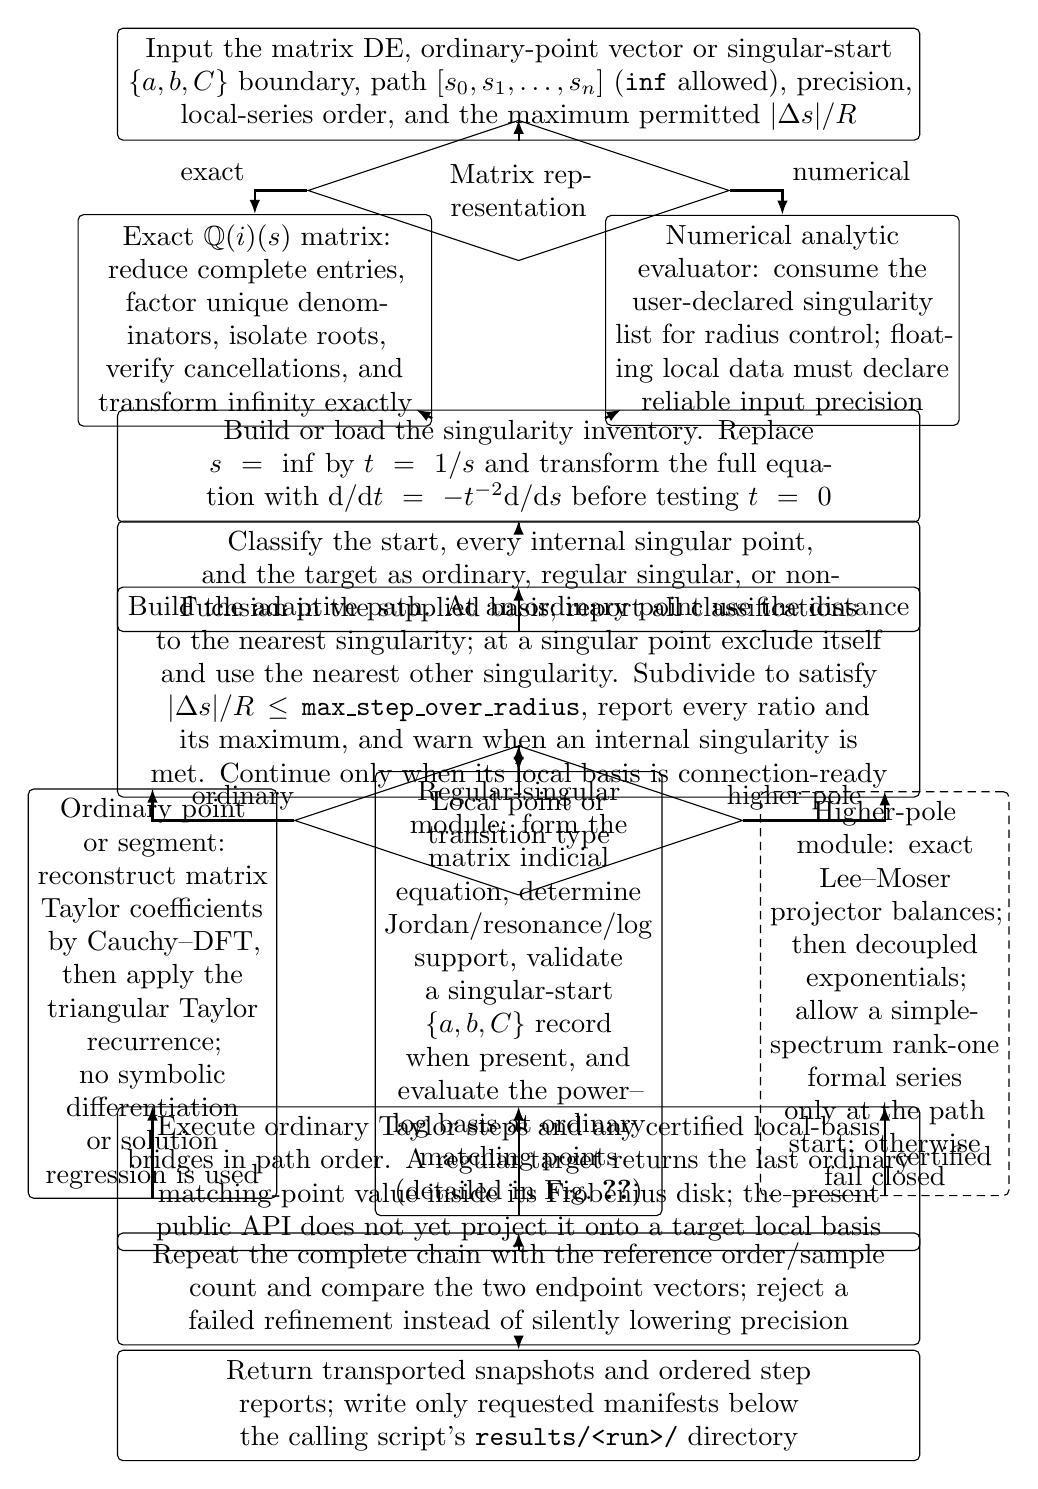
\begin{tikzpicture}[
  box/.style={draw, rounded corners=2pt, align=center, inner sep=3.5pt},
  decision/.style={draw, diamond, aspect=3.0, align=center, inner sep=1.2pt},
  flow/.style={-{Latex[length=1.8mm]}, thick},
  fail/.style={draw, rounded corners=2pt, align=center, inner sep=3.5pt, densely dashed}
]
\node[box, text width=.82\textwidth] (input) at (0,0)
  {Input the matrix DE, ordinary-point vector or singular-start $\{a,b,C\}$ boundary,
   path $[s_0,s_1,\ldots,s_n]$ (\texttt{inf} allowed), precision, local-series order,
   and the maximum permitted $|\Delta s|/R$};
\node[decision, text width=.25\textwidth] (representation) at (0,-1.35)
  {Matrix representation};
\node[box, text width=.35\textwidth] (exact) at (-3.35,-3.00)
  {Exact $\mathbb Q(i)(s)$ matrix: reduce complete entries, factor unique denominators,
   isolate roots, verify cancellations, and transform infinity exactly};
\node[box, text width=.35\textwidth] (numeric) at (3.35,-3.00)
  {Numerical analytic evaluator: consume the user-declared singularity list for radius
   control; floating local data must declare reliable input precision};
\node[box, text width=.82\textwidth] (inventory) at (0,-4.85)
  {Build or load the singularity inventory.  Replace $s=\mathrm{inf}$ by $t=1/s$ and
   transform the full equation with $\dd/\dd t=-t^{-2}\dd/\dd s$ before testing $t=0$};
\node[box, text width=.82\textwidth] (classify) at (0,-6.25)
  {Classify the start, every internal singular point, and the target as ordinary,
   regular singular, or non-Fuchsian in the supplied basis; report all classifications};
\node[box, text width=.82\textwidth] (path) at (0,-7.72)
  {Build the adaptive path.  At an ordinary point use the distance to the nearest
   singularity; at a singular point exclude itself and use the nearest other singularity.
   Subdivide to satisfy $|\Delta s|/R\leq\texttt{max\_step\_over\_radius}$, report every
   ratio and its maximum, and warn when an internal singularity is met.  Continue only when
   its local basis is connection-ready};
\node[decision, text width=.26\textwidth] (pointkind) at (0,-9.35)
  {Local point or transition type};
\node[box, text width=.24\textwidth] (ordinary) at (-4.65,-11.55)
  {Ordinary point or segment: reconstruct matrix Taylor coefficients by Cauchy--DFT,
   then apply the triangular Taylor recurrence; no symbolic differentiation or solution
   regression is used};
\node[box, text width=.28\textwidth] (regular) at (0,-11.55)
  {Regular-singular module: form the matrix indicial equation, determine
   Jordan/resonance/log support, validate a singular-start $\{a,b,C\}$ record when present,
   and evaluate the power--log basis at ordinary matching points
   (detailed in Fig.~\ref{fig:log-decision-route})};
\node[fail, text width=.24\textwidth] (nonfuchsian) at (4.65,-11.55)
  {Higher-pole module: exact Lee--Moser projector balances; then decoupled
   exponentials; allow a simple-spectrum rank-one formal series only at the path start;
   otherwise fail closed};
\node[box, text width=.82\textwidth] (transport) at (0,-13.90)
  {Execute ordinary Taylor steps and any certified local-basis bridges in path order.
   A regular target returns the last ordinary matching-point value inside its Frobenius disk;
   the present public API does not yet project it onto a target local basis};
\node[box, text width=.82\textwidth] (refine) at (0,-15.30)
  {Repeat the complete chain with the reference order/sample count and compare the two
   endpoint vectors; reject a failed refinement instead of silently lowering precision};
\node[box, text width=.82\textwidth] (output) at (0,-16.78)
  {Return transported snapshots and ordered step reports; write only requested manifests
   below the calling script's \texttt{results/<run>/} directory};

\draw[flow] (input) -- (representation);
\draw[flow] (representation) -| node[above left]{exact} (exact);
\draw[flow] (representation) -| node[above right]{numerical} (numeric);
\draw[flow] (exact) -- (inventory);
\draw[flow] (numeric) -- (inventory);
\draw[flow] (inventory) -- (classify);
\draw[flow] (classify) -- (path);
\draw[flow] (path) -- (pointkind);
\draw[flow] (pointkind) -| node[pos=.18,above]{ordinary} (ordinary.north);
\draw[flow] (pointkind) -- (regular);
\draw[flow] (pointkind) -| node[pos=.18,above]{higher pole} (nonfuchsian.north);
\draw[flow] (ordinary.south) -- (ordinary.south |- transport.north);
\draw[flow] (regular) -- (transport);
\draw[flow] (nonfuchsian.south) -- node[pos=.45,right]{certified} (nonfuchsian.south |- transport.north);
\draw[flow] (transport) -- (refine);
\draw[flow] (refine) -- (output);
\end{tikzpicture}
\caption{Basic numerical matrix-DE workflow.  Input formats and output layout are detailed
in Sec.~\ref{subsec:public-interface}; exact/numerical representations and ordinary
recurrences in Sec.~\ref{subsec:ordinary}; singularity inventory and infinity in
Sec.~\ref{subsec:singularity-inventory}; path construction and each $|\Delta s|/R$ report in
Sec.~\ref{subsec:path}; matrix indicial data in Sec.~\ref{subsec:frobenius}; the log node in
 Sec.~\ref{subsec:log}; the high-pole module and its fail-closed boundary in
 Sec.~\ref{subsec:nonfuchsian}; and
transport/refinement in Sec.~\ref{subsec:transport-api}.}
\label{fig:numerical-workflow}
\end{figure}

\section{Core function II: semi-analytic regulator-series reconstruction}
\label{sec:reconstruction-overview}

The second function reconstructs
\begin{equation}
 F(\eps)=\sum_{n=n_{\min}}^{m}f_n\eps^n+O(\eps^{m+1}),
\end{equation}
where the integer powers are analytic information and each $f_n$ is an arbitrary-precision
numerical vector.  Both $m$ and an upstream symbolically certified $n_{\min}$ are required;
the sample grid, working precision, and surplus fitted orders are automatic unless overridden. Every regulator
sample calls the complete basic solver of Fig.~\ref{fig:numerical-workflow}; no independent
solution-fitting DE engine exists.

\begin{figure}[p]
\centering
\footnotesize
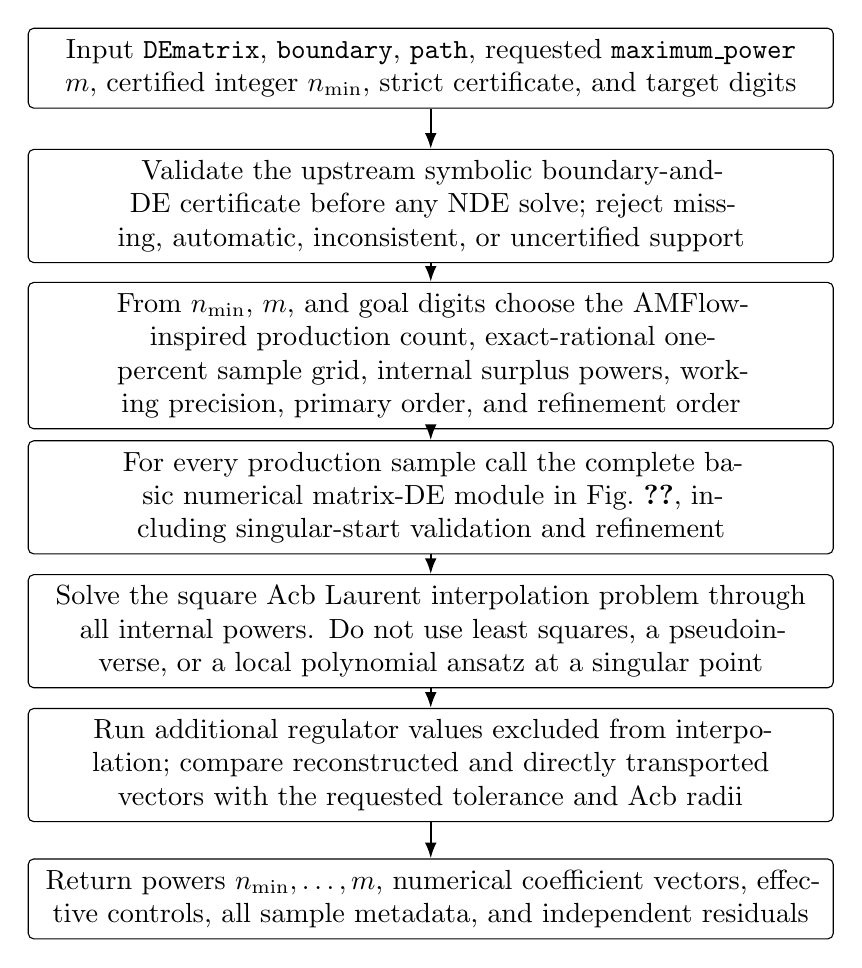
\begin{tikzpicture}[
  box/.style={draw, rounded corners=2pt, align=center, inner sep=4pt},
  decision/.style={draw, diamond, aspect=3.0, align=center, inner sep=1.5pt},
  flow/.style={-{Latex[length=2mm]}, thick}
]
\node[box, text width=.82\textwidth] (input) at (0,0)
  {Input \texttt{DEmatrix}, \texttt{boundary}, \texttt{path}, requested
   \texttt{maximum\_power} $m$, certified integer $n_{\min}$, strict certificate, and target digits};
\node[box, text width=.82\textwidth] (leading) at (0,-1.75)
  {Validate the upstream symbolic boundary-and-DE certificate before any NDE solve;
   reject missing, automatic, inconsistent, or uncertified support};
\node[box, text width=.82\textwidth] (plan) at (0,-3.65)
  {From $n_{\min}$, $m$, and goal digits choose the AMFlow-inspired production count,
   exact-rational one-percent sample grid, internal surplus powers, working precision,
   primary order, and refinement order};
\node[box, text width=.82\textwidth] (solve) at (0,-5.45)
  {For every production sample call the complete basic numerical matrix-DE module in
   Fig.~\ref{fig:numerical-workflow}, including singular-start validation and refinement};
\node[box, text width=.82\textwidth] (fit) at (0,-7.15)
  {Solve the square Acb Laurent interpolation problem through all internal powers.
   Do not use least squares, a pseudoinverse, or a local polynomial ansatz at a singular point};
\node[box, text width=.82\textwidth] (validate) at (0,-8.85)
  {Run additional regulator values excluded from interpolation; compare reconstructed and
   directly transported vectors with the requested tolerance and Acb radii};
\node[box, text width=.82\textwidth] (output) at (0,-10.55)
  {Return powers $n_{\min},\ldots,m$, numerical coefficient vectors, effective controls,
   all sample metadata, and independent residuals};

\draw[flow] (input) -- (leading);
\draw[flow] (leading) -- (plan);
\draw[flow] (plan) -- (solve);
\draw[flow] (solve) -- (fit);
\draw[flow] (fit) -- (validate);
\draw[flow] (validate) -- (output);
\end{tikzpicture}
\caption{Semi-analytic regulator-series workflow.  The basic NDE node is exactly
Fig.~\ref{fig:numerical-workflow} and is not expanded again.  The AMFlow error estimate,
automatic $\eps$ scale, surplus orders, precision rules, support certificate, square interpolation, and
validation are detailed in Sec.~\ref{subsec:reconstruction-details}; the complete optional
parameter list is in Table~\ref{tab:regulator-api} of Sec.~\ref{subsec:public-interface}.}
\label{fig:reconstruction-workflow}
\end{figure}

\section{Installation and dependencies}
\label{sec:installation}

The runtime requirements are only Python~$\geq3.10$ and
\texttt{python-flint>=0.6}.  After publication, install from the package index with
\begin{verbatim}
python -m pip install FlintNDE
\end{verbatim}
or install a downloaded source tree once with
\begin{verbatim}
python -m pip install path/to/package-FlintNDE/versions/FlintNDE-0.4.0
\end{verbatim}
Editable development mode uses the same command with \texttt{-e}.  A calling script may
then live in any directory and simply \texttt{import flintnde}; the package source is not
copied beside it.  When the caller passes \texttt{initialize\_output\_layout(\_\_file\_\_)},
all generated files are rooted beside that calling script, never in the installed package.
Importing the package initializes the global Acb context to 200 decimal working digits plus
32 guard bits.  Calling \texttt{configure\_working\_precision()} restores that default, while
an explicit positive integer overrides it.

The source tree also provides a standard Wolfram Language package.  Add the 0.4.0 version
root to \texttt{\$Path}, then evaluate
\begin{verbatim}
Needs["FlintNDE`"];
system = FlintNDERationalSystem[{{1/(x-1)}}, x];
plan = FlintNDEPlanPath[system, 0, {1/2},
  "WorkingPrecisionDigits" -> 100];
result = FlintNDEExecutePath[system, {1}, plan,
  "WorkingPrecisionDigits" -> 100];
\end{verbatim}
The planning default is \texttt{"SingularityMode" -> "Avoid"}; explicit
\texttt{"SingularityJump"} mode carries the branch warning.  These are the only accepted
mode values.  Messages use English by default and
\texttt{MessageLanguage -> "CN"} selects Chinese.

The Wolfram option \texttt{"WorkDirectory"} denotes the temporary runtime root itself.
Its \texttt{Automatic} value creates one \texttt{results\_temp/} below the current calling
directory, and the interface adds only a short \texttt{bridge/} child with 16-hex-token file
names.  It never appends a second \texttt{results\_temp} or a long task-specific directory.
On Windows, all complete request, output, and log paths are checked before any file write or
Python launch.  A path longer than 259 characters returns
\texttt{RuntimePathTooLong} with the actual path and length.  Request write failure,
missing \texttt{python-flint}, bridge launch failure, zero-exit missing output, and invalid
output are reported separately as \texttt{RuntimeInputWriteFailed},
\texttt{PythonFlintUnavailable}, \texttt{BridgeLaunchFailed},
\texttt{BridgeOutputMissing}, and \texttt{BridgeOutputInvalid}.

Independent fixed-regulator jobs use
\texttt{FlintNDE}\allowbreak\texttt{EvaluateEpBatch}, with the option
\texttt{Parallel}\allowbreak\texttt{TaskCount -> 12}.  The default upper bound is 12 worker processes; the
effective count is the smaller of that bound and the number of jobs, and queued jobs start
automatically as workers finish.  The Python counterparts are
\texttt{run\_ep\_tasks(..., parallel\_task\_count=12)} and the same
\texttt{parallel\_task\_count} option of \texttt{reconstruct\_series\_solution}.  This outer
process count is independent of python-flint's in-process \texttt{ctx.threads} setting.

The complete input syntax and every optional parameter are listed in
Sec.~\ref{subsec:public-interface}.

\section{Examples}
\label{sec:examples}

\subsection{Certified Laurent reconstruction}

The executable \texttt{examples/ep\_series\_reconstruction.py} uses the zero matrix DE and
the analytically known boundary
\begin{equation}
 Y(0,\epsilon)=\epsilon^{-1}+2+3\epsilon+4\epsilon^2+5\epsilon^3+6\epsilon^4.
\end{equation}
The upstream example certificate therefore states $n_{\min}=-1$.  FlintNDE validates that
certificate before any solve, but does not infer it from sampled values.  The user requests only
the finite part ($m=0$); the first square fit includes two additional powers.  With the deliberately
strict independent-point tolerance, a failed first round appends two production points while
reusing every old production and validation value.  The accepted result recovers the pole
coefficient $1$ and finite part $2$.  The example uses
\texttt{parallel\_task\_count=12}; the process pool automatically reduces the effective count
when fewer regulator tasks are available and queues excess tasks otherwise.

\subsection{de Sitter backend usage}

MadStree provides the physical de Sitter example at the upstream layer: it derives the symbolic
boundary and dlog DE, certifies the regulator support, and then calls this package.  FlintNDE does
not duplicate dS topology, master ordering, or normalization in a backend-only example.

\subsection{Schwarzschild two-ended radial system}
\label{subsec:qnm-example}

The retained cross-domain example starts from the odd-parity Regge--Wheeler function
$u^-_o$ in units $2M=1$:
\begin{equation}
 \frac{\dd^2u^-_o}{\dd x^2}
 +\frac{1}{x(x-1)}\frac{\dd u^-_o}{\dd x}
 +\left[\frac{\omega^2x^2}{(x-1)^2}
 -\frac{\ell(\ell+1)x-3}{x^2(x-1)}\right]u^-_o=0.
 \label{eq:qnm-original-rw}
\end{equation}
The even-parity function $u^+_o$ need not be assigned a second explicit equation here: at
fixed $(\ell,\omega)$ it is mapped to $u^-_o$ and its first derivative by the standard
Chandrasekhar--Darboux transformation \cite{Glampedakis:2017rar}.  The prefactor
\begin{equation}
 u^-_o=x^{\alpha_0}(x-1)^{\alpha_1 i\omega}u,
 \qquad (\alpha_0,\alpha_1)=(3,-1),
 \label{eq:qnm-u-transform}
\end{equation}
removes the second-order finite poles.  Writing $U=(u,u')^T$ and diagonalizing the constant
part with
\begin{equation}
 S_\infty=\begin{pmatrix}1&1\\ i\omega&-i\omega\end{pmatrix},
 \qquad U=S_\infty a,
\end{equation}
gives the explicitly organized first-order system
\begin{equation}
 \frac{\dd a}{\dd x}=\left[\Lambda_\infty+
 \frac{R_0}{x}+\frac{R_H}{x-1}\right]a,
 \qquad \Lambda_\infty=\begin{pmatrix}i\omega&0\\0&-i\omega\end{pmatrix},
 \label{eq:qnm-diagonal-system}
\end{equation}
where, with $\lambda=(\ell-1)(\ell+2)/2$ and $d=(\lambda-2)/\omega$,
\begin{align}
 R_0&=\begin{pmatrix}-5+id&id\\5-id&-id\end{pmatrix},\\
 R_H&=\begin{pmatrix}2+2i\omega-id&3-id\\-2-2i\omega+id&-3+id\end{pmatrix}.
 \label{eq:qnm-residue-matrices}
\end{align}
Thus no unreduced companion-matrix expression is needed by the example.

The physical meaning of the zero leading series coefficient must be read after the known
endpoint factors are removed.  Since $r_*\sim\log(x-1)$ at the horizon, the ingoing plane
wave $e^{-i\omega r_*}$ is absorbed by Eq.~\eqref{eq:qnm-u-transform}; its remaining
Frobenius series has indicial leading power zero.  At infinity, after extracting
$e^{\pm i\omega r_*}$ and the corresponding algebraic power in $z=1/x$, the outgoing or
incoming analytic remainder likewise starts at power zero.  These zero roots label the
regular remainders of asymptotic plane waves, not constant physical waves.

For the tabulated quasinormal frequency, the script starts literally at $x=1$ once and at
\texttt{inf} once, transports the selected branches to a common matching point, and
decomposes each vector in the opposite endpoint basis
\cite{Leaver:1985ax,Berti:2009kk}.  The forbidden-to-allowed ratios are
\begin{center}
\begin{tabular}{lcc}
\toprule
Frequency & horizon $\to$ infinity & infinity $\to$ horizon\\
\midrule
tabulated quasinormal frequency & $2.4549\times10^{-15}$ & $3.7235\times10^{-15}$\\
relative shift $10^{-3}$ & $3.9002\times10^{-3}$ & $5.9175\times10^{-3}$\\
\bottomrule
\end{tabular}
\end{center}
Infinity is first mapped to $z=1/x=0$.  Its $A_{-2}$ eigenvalues are simple and distinct, so
Eq.~\eqref{eq:formal-rank-one-recurrence} constructs the outgoing and incoming branches and
the nearest-root-gap rule with $q=3$ gives the first ordinary point $x\simeq74.20$.  At
reference order 55 the outgoing/incoming five-order block ratios are approximately
$0.02037$ and $0.02210$; neither branch has reached its least term in the available range.
Their local vectors agree with the independently implemented scalar second-order recurrence
to $1.2\times10^{-42}$ and $5.1\times10^{-42}$, respectively; the separate comparison at
$x=28$ remains better than $3\times10^{-18}$.  The more distant start amplifies Cauchy--DFT
aliasing between stiff exponential branches, so this example uses sampling-radius fraction
$0.40$; the maximum primary/reference transport difference is then $3.75\times10^{-22}$.
Hence the first table row is consistent with zero at the demonstrated
refinement scale, while the nonzero shifted row is a counterfactual boundary mismatch.  This
is a formal/Gevrey infinity expansion, not a convergent Frobenius disk.  The example tests a
radial connection problem only and introduces no integral-family assumption.

\section{Technical details}
\label{sec:technical-details}

\subsection{Matrix differential equations and ordinary points}
\label{subsec:ordinary}

We use the column-vector convention
\begin{equation}
  \frac{\dd}{\dd z}Y(z)=A(z)Y(z),
  \qquad A(z)\in\mathbb C^{N\times N}.
  \label{eq:matrix-system}
\end{equation}
At an ordinary point $c$, write $s=z-c$ and
\begin{equation}
  A(c+s)=\sum_{m\geq0}A_m(c)s^m,
  \qquad
  Y(c+s)=\sum_{n\geq0}Y_n(c)s^n.
\end{equation}
Substitution in Eq.~\eqref{eq:matrix-system} gives the triangular recurrence
\begin{equation}
  Y_{n+1}(c)=\frac{1}{n+1}\sum_{m=0}^{n}A_m(c)Y_{n-m}(c).
  \label{eq:ordinary-recurrence}
\end{equation}
The recurrence advances either one boundary vector or a complete fundamental matrix.  The
former is cheaper when only one physical boundary condition is required.

\subsubsection{General analytic matrix coefficients}

The default backend does not assume that $A(z)$ has only simple poles.  If $A$ is analytic
on and inside the circle $|s|=r$, Cauchy's formula gives
\begin{equation}
  A_m(c)=\frac{1}{2\pi r^m}\int_0^{2\pi}
  A(c+r e^{\mathrm i\theta})e^{-\mathrm i m\theta}\,\dd\theta.
\end{equation}
With $K$ equally spaced samples this becomes the discrete Fourier projection
\begin{equation}
  A_m^{(K)}(c)=\frac{1}{K r^m}\sum_{j=0}^{K-1}
  A(c+r\xi_K^j)\xi_K^{-jm},
  \qquad \xi_K=e^{2\pi\mathrm i/K}.
  \label{eq:cauchy-dft}
\end{equation}
This is a coefficient reconstruction from numerical matrix evaluations, not symbolic
differentiation and not a regression fit for the solution.  It applies equally to rational,
algebraic, and user-supplied analytic
matrix evaluators, provided the sampling circle lies in their common analytic domain.

For rational matrices, direct series division can later be supplied as an optional
coefficient generator.  Equation~\eqref{eq:cauchy-dft} remains the general default and a
common validation route.  The truncation and Fourier-aliasing error is monitored by a second
transport with higher Taylor order and more Cauchy samples.

\subsubsection{Exact singularity inventory and infinity}
\label{subsec:singularity-inventory}

For an exact Gaussian-rational input, each complete matrix entry is first reduced in
$\mathbb Q(i)[s]$ as
\begin{equation}
 A_{ij}(s)=\frac{N_{ij}(s)}{D_{ij}(s)},
 \qquad \gcd(N_{ij},D_{ij})=1.
\end{equation}
The finite candidate set is the union of roots of the reduced denominators.  A scalar
$a+ib$ is stored as two FLINT \texttt{fmpq} values, and an $N$-dimensional complex matrix as
two $N$-dimensional \texttt{fmpq\_mat} objects; no $2N$ real-block embedding is used.  Exact
$\mathbb Q(i)[s]$ arithmetic performs the polynomial gcd and square-free decomposition.  If a
square-free factor contains both the exact root zero and algebraic roots outside
$\mathbb Q(i)$, the factor $s$ is divided out first.  Hence the boundary point $s=0$ retains
its exact Gaussian-rational identity and remains eligible for exact Frobenius dispatch, while
the remaining roots are isolated as Acb balls.  The pole order recorded at a root is
the largest order among all entries of the \emph{complete} matrix.  A first-order pole of the
full matrix is Fuchsian.  An order greater than one certifies only
\texttt{non\_fuchsian\_input\_basis}; it is not, by itself, a basis-invariant proof of an
irregular singularity.  In particular, inspecting only diagonal entries is invalid, but a
higher-order off-diagonal entry may still be lowered by a meromorphic gauge or shearing
transformation.  Combining and reducing each complete entry before collecting denominators
is essential: terms with the same denominator may cancel, and a cancelled candidate must
not enter the inventory.

The point at infinity is tested in its own local variable.  With
\begin{equation}
 t=\frac{1}{s},\qquad \frac{\dd s}{\dd t}=-\frac{1}{t^2},
\end{equation}
Eq.~\eqref{eq:matrix-system} becomes
\begin{equation}
 \frac{\dd Y}{\dd t}=B(t)Y,
 \qquad B(t)=-\frac{1}{t^2}A\!\left(\frac{1}{t}\right).
 \label{eq:infinity-transform}
\end{equation}
Thus the pole order of the full $B$ at $t=0$, including the derivative Jacobian, tests
whether infinity is ordinary, Fuchsian, or non-Fuchsian in the transformed input basis.
For a reduced scalar entry with numerator and denominator degrees $n$ and $d$, its
contribution has pole order $\max(0,n-d+2)$.  Exact divisibility is both faster and stronger
than probing $A(p+\delta)$ for small numerical $\delta$; displaced evaluations are useful
diagnostics but cannot certify a cancellation or distinguish a small residue from zero.

After building this inventory, the package attempts an exact structural decomposition
\begin{equation}
 A(s)=P(s)+\sum_j\frac{R_j}{s-p_j},
 \label{eq:polynomial-simple-poles}
\end{equation}
where the matrix polynomial $P$ may have any finite degree.  The pole locations and residues
are derived internally; the caller need not supply a dlog alphabet.  The partial-fraction
recurrence is selected only if reconstruction of the complete matrix is exact and every
finite pole is simple.  A higher-order pole or any failed identity check remains on the
general rational-matrix route.  A pure polynomial system is the valid zero-finite-pole
subcase.  Thus Eq.~\eqref{eq:polynomial-simple-poles} is a certified optimization of the
generic interface, not a restriction to dlog differential equations.

\subsubsection{Path subdivision and precision}
\label{subsec:path}

At an ordinary point $c$, let $R(c)$ be the distance to the nearest finite singularity.  At
a singular point $p$, let
\begin{equation}
 R_{\mathrm{sing}}(p)=\min_{q\ne p}|p-q|,
\end{equation}
where the point itself is excluded.  The package uses
\begin{equation}
  |\Delta z|<r< R(c)
\end{equation}
for every segment.  A long path is subdivided according to a fixed fraction of $R(c)$.  The
primary and reference chains are evaluated independently.  Their final relative difference
is a truncation diagnostic; it is not confused with the radius carried by an individual
FLINT ball.  Multi-segment calculations restart from high-precision midpoints to limit
interval wrapping and are consequently reported as arbitrary-precision point transport,
not as a rigorous enclosure of the complete path.

The convergence radius and the step length are distinct quantities.  The singularity set
fixes $R(c)$ or $R_{\mathrm{sing}}(p)$; the user option
\texttt{max\_step\_over\_radius} only imposes
$|\Delta z|/R\leq f_{\mathrm{step}}$.  Planning and execution are separate operations:
a planner consumes raw user points and serializes all ordinary nodes, sample assignments,
singularity classifications, and bridge geometry; the executor restores that plan and must
not call the planner again.

The default mode is \texttt{singularity\_mode="avoid"}.  If a straight segment contains
an internal singularity, planning stops with a structured report naming both the singularity
and the affected user-point pair.  The caller can instead provide explicit detour points.
Any multipoint transport through intermediate nodes is called a jump in this manual.  Only
the explicit \texttt{"singularity\_jump"} mode builds a local-basis bridge across a
singularity; this operation is called a singularity jump.  No Boolean switch or alternate
mode spelling is accepted.  A singularity jump
chooses a branch of a multivalued local solution equivalent to one detour homotopy class;
the package reports this responsibility and the caller must confirm the branch.  The bridge
may use the original Frobenius system, a
Moser-reduced Fuchsian system, or a certified exponential-times-power--log sector.  A
high-pole checkpoint remains fail closed when none of these exact gates supplies a local
basis.

When a singularity jump is enabled, entering the step range of a pole creates incoming and outgoing
matching nodes.  Subsequent user points are inspected in order; the last point still within
one admissible pole-centred step becomes the next node.  If the first point is already
outside that range, one admissible step is taken towards it before ordinary planning resumes.
The incoming step is controlled by $R_{\mathrm{sing}}(p)$ of the target singularity, not by
the radius of the preceding ordinary point.

The global FLINT precision is
\begin{equation}
 p_{\mathrm{bit}}=\left\lceil p_{\mathrm{dec}}\log_2 10\right\rceil+32.
\end{equation}
For example, 70 and 100 decimal digits request 265 and 365 bits, and higher decimal requests
continue to increase the bit count by the same formula.  Segment projection, match ratios,
rotation factors, and winding/monodromy geometry are constructed at the current Arb
precision rather than in binary64.  Serialized plans record
\texttt{planning\_precision\_digits}; Acb coordinates are stored as Arb midpoint--radius--
exponent records.  Execution at a higher working precision than planning is rejected and
requires replanning, because serialization cannot recover discarded information.  Increasing
only the number of output digits does not change the working precision.
The Python import and all three Wolfram entry points default to 200 decimal digits, which gives
697 bits including the guard bits.

\small
\begin{longtable}{L{0.22\textwidth}L{0.72\textwidth}}
\caption{Execution contract for ordinary and singular path locations.}
\label{tab:path-location-contract}\\
\toprule
Path role & Implemented action, radius rule, and returned object \\
\midrule
\endfirsthead
\toprule
Path role & Implemented action, radius rule, and returned object \\
\midrule
\endhead
Ordinary start & The input is a finite Acb column.  Taylor transport starts at the stated
point, and its convergence radius is the distance to the nearest singularity. \\
Singular start & A regular singularity accepts an exact $\{a,b,C\}$ power--log record;
an exponential singularity accepts only an explicit $\{\phi,a,b,C\}$ record.  Neither is
a finite value at the singularity.  The package validates the indicial, exponential, and log
branch, evaluates it at the first ordinary matching point, and then starts Taylor transport.
The matching distance is limited by $R_{\rm sing}$, which excludes the singularity itself.
For an exponential solution, FlintNDE derives the exact sector from the DE and verifies
$\phi$; it never infers a missing exponential signature from $C$. \\
Ordinary target & The last snapshot is the transported Acb column at the stated target. \\
Regular-singular target & The executable list ends at an ordinary matching point inside the
target Frobenius disk; it never invents a finite value at the singularity.  The target
classification, singular point, matching point, and match-distance ratio are reported.  If
the target coordinate carries the save tag and a direct regular-singular power--log basis is
available, FlintNDE solves for and writes reusable $\{a,b,C\}$ coefficients.  These are local
boundary data, not a finite value at the singularity. \\
Internal regular singularity & The path stores ordinary matching points on both sides and a
Frobenius bridge between them.  Both match-to-singularity distances are divided by the
singularity radius $R_{\rm sing}$, not by either neighboring ordinary-point radius.  The
principal Acb log/power branch and both ratios are reported. \\
Higher-pole checkpoint & The inventory first records
\texttt{non\_fuchsian\_input\_basis}.  The local dispatcher tries exact Lee--Moser
projector balances and then the certified decoupled exponential-sector gate.
A successful route uses
the same two-sided local bridge and returns the original integral basis.  Otherwise
continuation fails closed; an internal point may instead be avoided with explicit ordinary
detour points.  A continuation-ready exponential checkpoint tagged by
\texttt{(coordinate,"save")} writes reusable $\{\phi,a,b,C\}$ data at the bridge. \\
Infinity & The complete equation is first transformed to $t=1/s$, including the
$-t^{-2}$ Jacobian.  The resulting point $t=0$ then follows the same ordinary,
regular-singular, or non-Fuchsian-input-basis rules; its local radius is measured to the
nearest other singularity in the transformed variable. \\
\bottomrule
\end{longtable}
\normalsize

\subsubsection{Capability preflight and the fail-closed boundary}

Before transport, \texttt{build\_adaptive\_path\_plan} applies the same local dispatcher to
both endpoints and every internal singular checkpoint.  Its
\texttt{continuation\_ready} flag is a capability gate, not an accuracy estimate.  If it is
false, the plan records the singularity classification, attempted certified route, and the
missing structure (for example a ramified or defective formal block, an algebraic extension,
or a Stokes connection).  The caller must then choose ordinary detour points or supply external
local connection data.  The numerical transport must not be started on that plan.

This gate applies to every nonordinary checkpoint, not only to a high-order pole.  A regular
singularity whose center is outside $\mathbb Q(i)$, or whose exact indicial, Jordan, or
resonance structure is unsupported by the present power--log constructor, also sets
\texttt{continuation\_ready=False}.  The direct path builder reports the point kind and the
failed local-basis reason instead of postponing the failure until transport.

A direct call to the path builder enforces the same rule.  It raises
\texttt{LocalReductionError} before transport.  In particular, failure of the exact, Lee--Moser, exponential,
or rank-one formal gates never falls back to an ordinary Taylor/Cauchy expansion.  The sole
start-only formal route initializes a solution from the singular boundary to a first ordinary
matching point in one Stokes sector; it is not continuation-ready when the same point is
internal or the target.

\subsubsection{Coordinate-only save tags}

A saved path point has no user-supplied name.  Its input is exactly
\texttt{(coordinate, "save")}; for example,
\begin{verbatim}
path = [(z0, "save"), z1, (z2, "save")]
transport_path_refined(system, boundary, path)
\end{verbatim}
The same pair may be used for adaptive-path start, target, or detour coordinates.  A singular
middle coordinate is accepted only with this tag; it denotes a saved singular checkpoint,
not an ordinary detour.  Internal \texttt{NamedPoint} labels remain routing diagnostics and
are not part of the save contract.

On reaching a tagged coordinate, FlintNDE immediately writes
\texttt{flintnde\_save\_001.json}, \texttt{flintnde\_save\_002.json}, and so on in path
order.  The default directory is the caller's \texttt{Path.cwd()};
\texttt{save\_output\_directory} may select another caller-owned directory.  Only after all
transport steps succeed does the package write \texttt{flintnde\_save\_points.json}.  Thus a
later failure preserves completed point files without claiming a complete summary.  A
refined transport writes the reference chain only.

At an ordinary point the record contains the coordinate and the transported Acb column.  At
a direct regular singular start or target it contains reusable $\{a,b,C\}$ terms and
\texttt{resultType=frobenius\_boundary}.  A certified decoupled exponential start, target, or
middle bridge instead contains $\{\phi,a,b,C\}$ and
\texttt{resultType=exponential\_boundary}.  These are boundary data, not $Y(z_*)$.
A start-only formal exponential branch may be saved at the start and records
\texttt{continuationReady=false}; the same method remains forbidden internally or at the
target.  Saving a Lee--Moser transformed original-basis singularity still requires a
certified inverse local jet, and unsupported Stokes connections remain fail closed.

\subsection{Regular singular points and the matrix indicial equation}
\label{subsec:frobenius}

Near $z=0$, consider a Fuchsian system
\begin{equation}
  \frac{\dd Y}{\dd z}
  =\left(\frac{R}{z}+\sum_{m\geq0}A_m z^m\right)Y.
  \label{eq:fuchsian-system}
\end{equation}
For $Y=z^\rho\sum_{n\geq0}v_nz^n$, the leading equation is
\begin{equation}
  (\rho\Id-R)v_0=0,
  \qquad
  \det(\rho\Id-R)=0.
  \label{eq:matrix-indicial}
\end{equation}
Equation~\eqref{eq:matrix-indicial} is the matrix indicial equation.  It is unnecessary to
eliminate the system to a scalar higher-order equation before determining its local
exponents.  For a semisimple nonresonant branch, the higher coefficients obey
\begin{equation}
  \bigl((\rho+n)\Id-R\bigr)v_n
  =\sum_{m=0}^{n-1}A_m v_{n-1-m}.
  \label{eq:frobenius-recurrence}
\end{equation}
See Ref.~\cite{Moriello:2019yhu} for a Feynman-integral implementation of generalized
series and their continuation.

\subsection{When logarithms are required}
\label{subsec:log}

The presence of a repeated indicial root is not, by itself, a criterion for logarithms.
There are two distinct mechanisms.

\subsubsection{Non-semisimple residue}

Suppose a single-root block is $R=\rho\Id+N$, with $N$ nilpotent.  Already for the leading
system one has
\begin{equation}
  z^R=z^\rho e^{N\log z}
  =z^\rho\sum_{q=0}^{\nu-1}\frac{N^q}{q!}(\log z)^q,
  \label{eq:jordan-log}
\end{equation}
where $N^\nu=0$.  A Jordan block of length $\nu$ therefore produces logarithms up to degree
$\nu-1$.  By contrast, a repeated but semisimple eigenvalue has $N=0$ and produces no log
through this mechanism.

\subsubsection{Integer-difference resonance}

Even for a diagonalizable residue, Eq.~\eqref{eq:frobenius-recurrence} becomes singular if
$\rho+n$ is another indicial root.  Let $P_{\rho+n}$ be the exact spectral projector onto
that eigenspace and let $b_n$ denote the right-hand side.  A pure-power recurrence exists
only if
\begin{equation}
  P_{\rho+n}b_n=0.
  \label{eq:resonance-compatibility}
\end{equation}
If this compatibility condition fails, the defect is transferred to a logarithmic
coefficient.  The package evaluates Eq.~\eqref{eq:resonance-compatibility} with exact
rational matrices.  The default route never silently substitutes a floating-point threshold
for this exact decision; the explicit numerical route described below records its full
threshold provenance.

\subsubsection{Unified power--log recurrence}

Write
\begin{equation}
  Y=z^\rho\sum_{n\geq0}\sum_{q=0}^{q_{\max}}
  v_{n,q}z^n(\log z)^q.
\end{equation}
At fixed $(n,q)$ the recurrence has the form
\begin{equation}
  \bigl((\rho+n)\Id-R\bigr)v_{n,q}
  +(q+1)v_{n,q+1}
  =\sum_{m=0}^{n-1}A_m v_{n-1-m,q}.
  \label{eq:power-log-recurrence}
\end{equation}
The default implementation uses FLINT rational matrices to create an exact manifest
containing roots, Jordan nilpotency, spectral projectors, initial eigenvectors, and every
active resonance gate.  FLINT then evaluates Eq.~\eqref{eq:power-log-recurrence} at the
  requested precision.  Exact classification is the default and never falls back to a
  threshold decision after an exact failure.  Only floating-point input selects the
  numerical gate, which uses
\begin{equation}
  \tau_{\rm rel}=N\,10^{-p},
  \qquad
  \tau_{\rm abs}=\tau_{\rm rel}
  \max\!\left(\max_{i,j}|R_{ij}|,\max_{m,i,j}|(A_m)_{ij}|\right),
  \label{eq:numerical-log-threshold}
\end{equation}
where $N$ is the system dimension (a conservative rank upper bound) and $p$ is the reliable
decimal input precision, not merely the arithmetic working precision.  Python binary64
input is capped at 15 decimal digits.  Higher-precision decimal or Acb input must carry or
declare its reliable precision; otherwise classification fails closed.  The user may replace
$\tau_{\rm rel}$.  Its manifest and mandatory warning report the matrix scale, both
thresholds, and the largest zeroed and smallest retained quantities in absolute units and
relative to the matrix scale.  A zero matrix scale is reported explicitly, with undefined
relative ratios rather than a fabricated number.  This threshold route is explicitly
 numerical rather than an exact certificate.  Ambiguous mixed-root defective systems fail
 closed.

Figure~\ref{fig:log-decision-route} summarizes the implemented decision route.  The
non-semisimple and resonance mechanisms are cumulative: a Jordan logarithm does not skip
the later resonance checks.
\begin{figure}[htbp]
\centering
\footnotesize
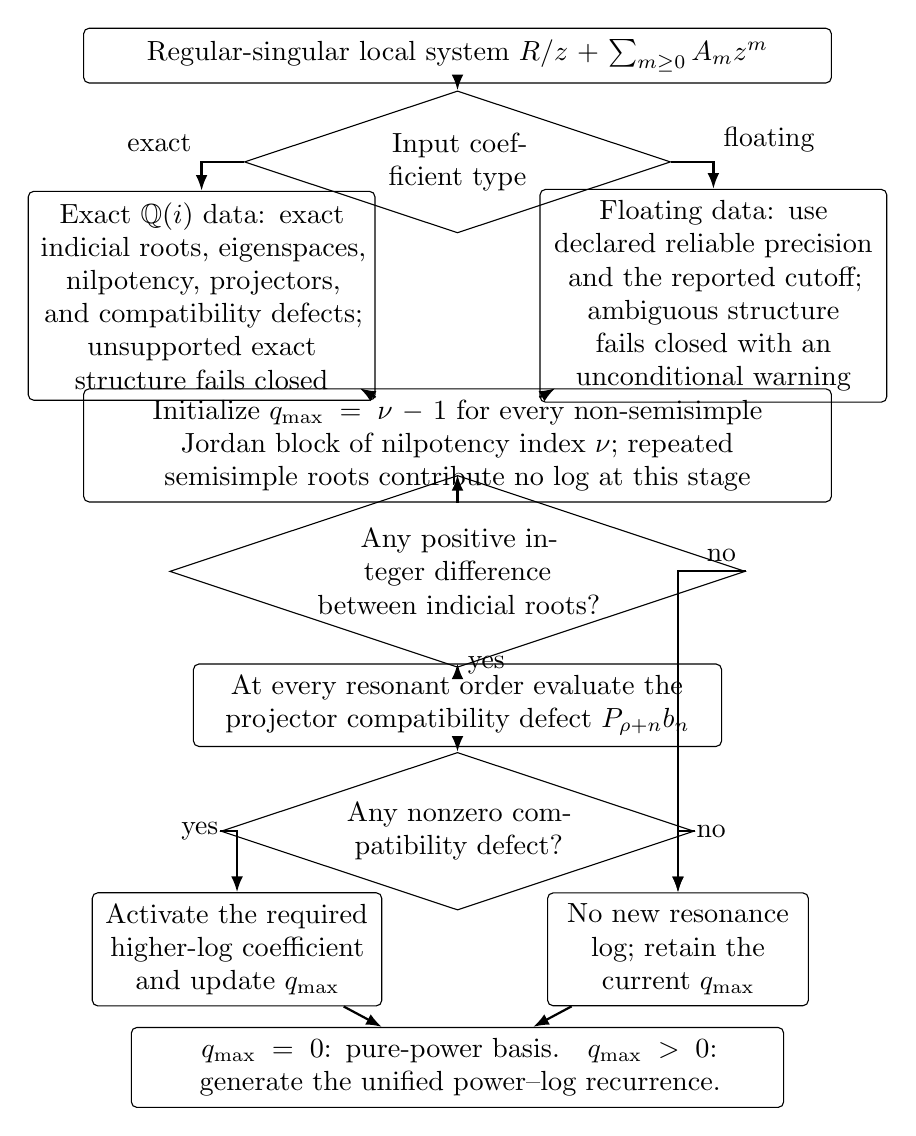
\begin{tikzpicture}[
  box/.style={draw, rounded corners=2pt, align=center, inner sep=4pt},
  decision/.style={draw, diamond, aspect=3.0, align=center, inner sep=1.5pt},
  flow/.style={-{Latex[length=2mm]}, thick}
]
\node[box, text width=.76\textwidth] (input) at (0,0)
  {Regular-singular local system $R/z+\sum_{m\geq0}A_mz^m$};
\node[decision, text width=.23\textwidth] (kind) at (0,-1.35)
  {Input coefficient type};
\node[box, text width=.34\textwidth] (exact) at (-3.25,-3.05)
  {Exact $\mathbb Q(i)$ data: exact indicial roots, eigenspaces, nilpotency,
   projectors, and compatibility defects; unsupported exact structure fails closed};
\node[box, text width=.34\textwidth] (numeric) at (3.25,-3.05)
  {Floating data: use declared reliable precision and the reported cutoff; ambiguous
   structure fails closed with an unconditional warning};
\node[box, text width=.76\textwidth] (classify) at (0,-4.95)
  {Initialize $q_{\max}=\nu-1$ for every non-semisimple Jordan block of nilpotency
   index $\nu$; repeated semisimple roots contribute no log at this stage};
\node[decision, text width=.30\textwidth] (integer) at (0,-6.55)
  {Any positive integer difference between indicial roots?};
\node[box, text width=.53\textwidth] (compatibility) at (0,-8.25)
  {At every resonant order evaluate the projector compatibility defect
   $P_{\rho+n}b_n$};
\node[decision, text width=.28\textwidth] (defect) at (0,-9.85)
  {Any nonzero compatibility defect?};
\node[box, text width=.28\textwidth] (activate) at (-2.80,-11.35)
  {Activate the required higher-log coefficient and update $q_{\max}$};
\node[box, text width=.25\textwidth] (unchanged) at (2.80,-11.35)
  {No new resonance log; retain the current $q_{\max}$};
\node[box, text width=.66\textwidth] (output) at (0,-12.85)
  {$q_{\max}=0$: pure-power basis.\quad $q_{\max}>0$: generate the unified
   power--log recurrence.};

\draw[flow] (input) -- (kind);
\draw[flow] (kind) -| node[above left]{exact} (exact);
\draw[flow] (kind) -| node[above right]{floating} (numeric);
\draw[flow] (exact) -- (classify);
\draw[flow] (numeric) -- (classify);
\draw[flow] (classify) -- (integer);
\draw[flow] (integer) -- node[right]{yes} (compatibility);
\draw[flow] (integer.east) -| node[pos=.18,above]{no} (unchanged.north);
\draw[flow] (compatibility) -- (defect);
\draw[flow] (defect) -| node[pos=.25,left]{yes} (activate.north);
\draw[flow] (defect) -| node[pos=.25,right]{no} (unchanged.north);
\draw[flow] (activate) -- (output);
\draw[flow] (unchanged) -- (output);
\end{tikzpicture}
\caption{Exact-first and precision-aware numerical routes for deciding logarithmic support.}
\label{fig:log-decision-route}
\end{figure}

 Once either gate activates a logarithmic sector, the local solution is always generated by
Eq.~\eqref{eq:power-log-recurrence}.  The package has no singular-point path that regresses a
pure polynomial solution and thereby drops a logarithmic branch.  The Laurent fit in
Section~\ref{sec:regulator-reconstruction} concerns regulator dependence only and is not a
local-solution ansatz.

\subsection{Non-Fuchsian input bases and genuine irregularity}
\label{subsec:nonfuchsian}

The test must use the complete matrix, not only its diagonal.  Nevertheless, finding a pole
of order two or higher in any entry proves only that the supplied basis is non-Fuchsian.
Meromorphic gauge transformations, including shearing transformations, can lower the pole
order and can remove a high-order off-diagonal term.  FlintNDE therefore applies the
following three-stage local dispatcher; the inventory label itself remains conservative.

First it applies the exact Lee--Moser reduction.  At a pole of order $p+1>1$, write
\begin{equation}
 A(z)=z^{-p-1}\bigl(A_0+zA_1+O(z^2)\bigr).
\end{equation}
The package constructs exact nilpotent Jordan chains of $A_0$, uses $A_1$ to resolve the
chain projector, and forms
\begin{equation}
 T_Q(z)=\Id-Q+\frac{Q}{z},\qquad
 T_Q^{-1}(z)=\Id-Q+zQ,\qquad Q^2=Q.
 \label{eq:moser-balance}
\end{equation}
For $I=T_QJ$ the complete transformed matrix is
\begin{equation}
 A_{\rm new}=T_Q^{-1}A T_Q-T_Q^{-1}T_Q'.
 \label{eq:moser-transformed-system}
\end{equation}
Every operation is performed over $\mathbb Q(i)$.  A balance is retained only when exact
idempotency holds and the pole order of the complete transformed matrix strictly decreases.
The leading two Laurent matrices are then recomputed and the procedure is repeated until the
system is Fuchsian.  The manifest stores the ordered projectors and the complete pole-order
history; applying all inverse balances to the final system must reproduce every original
rational matrix entry exactly.  A non-nilpotent highest Laurent matrix is an exact obstruction
to a Fuchsian gauge in this unramified meromorphic class.  Failure of an internal construction
assumption is instead reported as inconclusive, not as genuine irregularity.

Local power--log solutions are evaluated in the reduced basis and multiplied by the complete
product $T_{Q_1}\cdots T_{Q_m}$ before being returned.  A singular-start $\{a,b,C\}$ record is
validated directly in the original integral basis: FlintNDE generates an exact finite jet of
the reduced Frobenius basis, multiplies the whole jet by the Laurent gauge, sets all earlier
powers and higher logarithms to zero, and matches the requested coefficient $C$.  This is
necessary because a neighboring series coefficient can contribute to the original-basis
leading vector under a non-diagonal balance.

If a higher pole remains, FlintNDE attempts a restricted exponential route.  Suppose one
exact constant basis over $\mathbb Q(i)$ makes all higher Laurent matrices diagonal and
separates the system into sectors with identical diagonal high-pole signatures.  For one
such sector write
\begin{equation}
  A_{\rm high}(z)=\sum_{m=2}^{p}\frac{c_m}{z^m}\,\Id.
\end{equation}
With $Y=e^{\Phi(z)}U$, direct substitution gives
\begin{equation}
  \Phi'(z)=\sum_{m=2}^{p}c_m z^{-m},\qquad
  \Phi(z)=-\sum_{m=2}^{p}\frac{c_m}{m-1}z^{-(m-1)}.
  \label{eq:implemented-exponential-factor}
\end{equation}
The remaining equation for $U$ must have pole order at most one, after which the ordinary
power--log machinery applies unchanged.  In particular, $A_{-2}=k$ gives
$e^{-k/z}$.  A computed $k=0$ means only that this scalar exponential is absent; it does not
remove a nilpotent, defective, or off-diagonal higher-pole constraint.  Such a block must
still pass Moser reduction or a more general formal reduction.

The exactly decoupled gate remains deliberately strict.  It rejects a defective leading
matrix, a spectrum outside $\mathbb Q(i)$, non-diagonal higher Laurent matrices in the
selected basis, coupling between different exponential signatures, or a residual higher
pole after subtraction.  A boundary still uses $\{a,b,C\}$ for the power--log factor.  The
exact transformed $C$ selects the exponential sector automatically; if one term spans
several sectors the user must split it into separate terms.

There is one additional, explicitly formal route.  For pole order exactly two, suppose
$A_{-2}$ has $N$ simple distinct eigenvalues $k_j$ in $\mathbb Q(i)$.  For each right/left
eigenvector pair $(v_0,\ell)$ FlintNDE constructs
\begin{equation}
 Y=e^{-k/z}z^\rho\sum_{n=0}^{N_{\rm form}}v_nz^n,
 \qquad
 \rho=\frac{\ell^T A_{-1}v_0}{\ell^Tv_0}.
 \label{eq:formal-rank-one-ansatz}
\end{equation}
Equating the coefficient of $z^{\rho+q-2}$ gives
\begin{equation}
 (k\Id-A_{-2})v_q=
 \left[A_{-1}-(\rho+q-1)\Id\right]v_{q-1}
 +\sum_{m=0}^{q-2}A_m v_{q-2-m}.
 \label{eq:formal-rank-one-recurrence}
\end{equation}
The left-eigenvector compatibility at order $q+1$ fixes the otherwise free $v_0$ component
of $v_q$.  All eigenvectors, $\rho$, compatibility tests, and recurrence solves are exact in
$\mathbb Q(i)$; no numerical rank cutoff, least squares, or polynomial regression is used.
The public boundary remains $\{a,b,C\}$: presently $b=0$, $a=\rho$, and the exact vector $C$
must select one leading eigendirection.  The user does not enter $k$ separately.

The occurrence of $e^{-k/z}$ does not by itself imply divergence.  In the decoupled route,
after the complete scalar high-pole part is removed, a residual system with at most a simple
pole gives a convergent Frobenius power--log series whose disk is bounded by the nearest other
singularity.  By contrast, the recurrence in Eq.~\eqref{eq:formal-rank-one-recurrence} is in
general a sectorial Gevrey/asymptotic series.  FlintNDE always evaluates through the requested
degree $N$ and generates five additional coefficient vectors for diagnostics; it does not
silently replace $N$ by the observed least-term degree.  Define $T_n=v_nz^n$ and
$S_N=\sum_{n=0}^{N}T_n$.  The reported five-order block ratio and relative refinement are
\begin{equation}
 r_5=\frac{\left\|\sum_{j=1}^{5}T_{N+j}\right\|_\infty}
 {\left\|\sum_{j=0}^{4}T_{N-j}\right\|_\infty},
 \qquad
 \delta_5=\frac{\|S_{N+5}-S_N\|_\infty}{\|S_{N+5}\|_\infty}.
 \label{eq:formal-five-order-test}
\end{equation}
The five vector terms are summed before the infinity norm is taken.  The desired decreasing-block
condition is $r_5<1$.  Failure does not suppress the result: FlintNDE emits a conspicuous warning
and records the issue.  The actual value is always reported, including when it is below one, so
the user can judge whether the decrease is sufficient.  The report also retains the least-term
degree and magnitude as auxiliary information and says whether that degree was reached.
For a caller that already owns scalar terms, the public
\texttt{five\_term\_tail\_diagnostic} instead evaluates
\begin{equation}
 r_{5,\mathrm{scalar}}=
 \frac{\left|\sum_{j=1}^{5}T_{N+j}\right|}
 {\sum_{j=0}^{4}\left|T_{N-j}\right|}.
 \label{eq:public-scalar-five-order-test}
\end{equation}
The returned \texttt{FiveTermTailDiagnostic} exposes the numerator, denominator, ratio,
caller-supplied threshold, and strict pass flag.  This scalar diagnostic does not replace
Eq.~\eqref{eq:formal-five-order-test}; a zero denominator or an interval comparison that cannot
certify the strict inequality fails closed.
Generalized local expansions in Feynman-integral differential equations are discussed in
Ref.~\cite{Moriello:2019yhu}.

Thus ``how far from the irregular point may one evaluate?'' has two different answers.  The
residual-Fuchsian case uses $|z|<R_{\rm sing}$ and the normal configurable step fraction.  A
formal asymptotic branch has no convergence radius.  For automatic path generation FlintNDE
uses the separation of the exponential roots.  For sector $i$, define
\begin{equation}
 \Delta_i=\min_{j\ne i}|k_i-k_j|,
 \qquad
 \widehat n_{\min,i}(z)\simeq\frac{\Delta_i}{|z|}.
 \label{eq:formal-root-gap-estimate}
\end{equation}
This is the standard leading late-term estimate associated with the nearest competing
exponential action.  If $N$ is the requested formal-series order and $q>1$ is a safety factor,
the proposed distance is
\begin{equation}
 |z|_{\rm root}=\min_i\frac{\Delta_i}{qN}.
 \label{eq:formal-root-gap-point}
\end{equation}
The default is $q=3$, so $N$ is approximately one third of the estimated least-term degree.  For more
than two roots, each branch uses its nearest other root and the smallest proposed distance is
taken.  A one-root scalar high-pole sector is handled by the exactly decoupled exponential
power--log route rather than this formal root-gap rule.  The path interval and
\texttt{max\_step\_over\_radius}$\,R$ may only reduce the distance; the latter is applied only
when it gives a smaller step.  Final acceptance is nevertheless based on the actual tests in
Eq.~\eqref{eq:formal-five-order-test}; the root-gap estimate is not a proof of convergence or
accuracy.

The distance to the nearest other singularity is therefore only a reference scale, not a
convergence radius.  The user must remain in one Stokes sector and verify order and
matching-point stability.  User-supplied first matching points receive the same five-order
report and warning.  The
formal route is therefore allowed only as the path start.  An internal or target use is
rejected because FlintNDE has no Stokes matrix with which to connect the two sides.

\Needspace{10\baselineskip}
AMFlow provides a concrete engineering reference for the reducible part of this problem
\cite{Liu:2022chg,Huang:2026rjb}.  Its DE solver first decomposes the matrix into blocks.  On
each diagonal block it iteratively constructs a projector from the leading two local
coefficients and applies a balance transformation until the Poincar\'e rank vanishes; it then
uses shearing transformations to normalize residue eigenvalues.  The remaining
off-diagonal high-order blocks are reduced by solving linear matrix equations, after which
the transformed boundary is passed to the singular Frobenius solver.  If the leading matrix
has a nonzero Jordan eigenvalue, the projector route declares the positive Poincar\'e rank
irreducible and aborts.  FlintNDE now implements the exact local projector-balance iteration
on the complete matrix, including ordered projectors and a full rational-system round trip.
It does not reproduce AMFlow's global block decomposition, residue normalization, or separate
off-diagonal block solver; those are normalization and global-organization layers beyond the
local question of whether the supplied pole can be reduced to Fuchsian form.

More general irregular systems require sectors of the form
\begin{equation}
  Y(z)=e^{\Phi(z)}z^\rho
  \sum_{n,q}v_{n,q}z^n(\log z)^q,
  \qquad
  \Phi(z)=\sum_{j\geq1}\phi_j z^{-j}.
  \label{eq:irregular-ansatz}
\end{equation}
The implemented convergent scalar-sector case is
Eq.~\eqref{eq:implemented-exponential-factor}; the start-only simple-spectrum case is
Eq.~\eqref{eq:formal-rank-one-recurrence}.  Repeated/defective leading roots, higher
Poincar\'e rank, ramification, algebraic field extensions, general formal block gauges, and
Stokes matrices are not implemented.  The dispatcher fails closed whenever those data would
be needed; it never accepts ``set $k=0$'' as a substitute for the missing reduction.

\subsection{Numerical reconstruction in a regulator}
\label{sec:regulator-reconstruction}
\label{subsec:reconstruction-details}

Many dimensionally regulated calculations require coefficients of
\begin{equation}
  F(\eps)=\sum_{n=n_{\min}}^{n_{\max}}f_n\eps^n+O(\eps^{n_{\max}+1}).
\end{equation}
Instead of truncating every intermediate expression in $\eps$, one may solve the complete
numerical problem at several small exact-rational values $\eps_j$ and reconstruct the final
Laurent coefficients.  AMFlow uses this strategy \cite{Liu:2022chg}.

If the target coefficient has order $m$, $N+1$ samples lie at radius $r$, and the nearest
unaccounted singularity is at scale $R$, the estimate quoted in the AMFlow analysis is
\begin{equation}
  E_n\sim\left(\frac rR\right)^{N+1-n},
  \qquad
  N\sim m-1+\frac{\log E}{\log(r/R)}.
  \label{eq:amflow-error-estimate}
\end{equation}
If a single solve to error $p$ costs $t(p)\sim(-\log p)^\alpha$, the reference optimization is
\begin{equation}
  r\sim R E^{1/(\alpha m)},
  \qquad N\sim(\alpha+1)m-1,
  \qquad p\lesssim E^{(\alpha+1)/\alpha}.
  \label{eq:amflow-optimal-estimate}
\end{equation}
These are guidance formulas, not a posteriori proofs.

AMFlow 2.0 uses an empirical configuration \cite{Huang:2026rjb} in which $L$ is the number
of loops and the
assumed leading Laurent power is $n_{\min}=-2L$.  Its argument called ``order'' is the
reconstruction depth $K$ measured upward from $n_{\min}$, not the absolute highest power.
For decimal goal $g$,
\begin{align}
  N_{\mathrm sample}&=\left\lceil\frac52K+2L\right\rceil,\\
  \alpha_\eps&=\frac L2+\frac{g}{K+1},\\
  \eps_0&\simeq10^{-\alpha_\eps},
  &\eps_j&=\eps_0\left(1+\frac{j}{100}\right),\quad j=1,\ldots,N_{\mathrm sample},\\
  p_0&=\max\left(\left\lceil(N_{\mathrm sample}+2L)\alpha_\eps\right\rceil,30\right),\\
  p_{\mathrm work}&=\left\lceil2(1+p_{\mathrm extra})p_0\right\rceil.
  \label{eq:amflow-default-config}
\end{align}
The corresponding solver settings are $X_{\rm order}=4p_0$ and
$X_{\rm extra}=\lceil\max(50,p_0/5)\rceil$.  The one-percent spacing, rationalization of
sample points, doubled working precision, and these two expansion orders are implementation
choices in AMFlow 2.0 rather than consequences of Eqs.~\eqref{eq:amflow-error-estimate} and
\eqref{eq:amflow-optimal-estimate}.
FlintNDE implements the automatic choice as
$\max(200,\lceil2(1+p_{\mathrm extra})p_0\rceil)$.  The 200-digit lower bound is a
FlintNDE default rather than part of the quoted AMFlow formula; an explicit
\texttt{working\_precision\_digits} value overrides automatic planning.

The FlintNDE interface should not require a loop count: $L$ is specific to the Feynman
integral pole bound used by AMFlow and is not an intrinsic parameter of a general matrix
differential equation.  Nor can a finite collection of numerical regulator solves prove the
Laurent support of arbitrary Python callables.  The current interface therefore requires an
integer $n_{\min}$ together with a strict upstream certificate whose status is certified,
whose recorded integer agrees with $n_{\min}$, and whose method identifies the symbolic
boundary-and-DE analysis.  Missing certificates, automatic leading powers, and inconsistent
integers fail before any NDE solve.  MadStree produces this certificate automatically from its
physical boundary and dlog DE; FlintNDE remains independent of those physical data structures.

Let the certified global leading power be $n_{\min}$, let the user request the absolute
highest power $m$, and define
\begin{equation}
  P=\max(0,-n_{\min}),\qquad K=m-n_{\min}.
\end{equation}
The automatic production plan uses the AMFlow 2.0 formula after the transparent replacements
$2L\to P$ and $L/2\to P/4$:
\begin{align}
 N_{\mathrm fit}&=
 \max\!\left(\left\lceil\frac52K+P\right\rceil,K+1\right),\\
 \alpha_\eps&=\frac P4+\frac{g}{K+1},
 &\eps_0&\simeq10^{-\alpha_\eps},\\
 p_0&=\max\left(\left\lceil(N_{\mathrm fit}+P)\alpha_\eps\right\rceil,30\right),
 &p_{\mathrm work}&=\left\lceil2(1+p_{\mathrm extra})p_0\right\rceil.
  \label{eq:ndes-series-reconstruction-default}
\end{align}
All $N_{\mathrm fit}$ production samples are used in a square interpolation from
$n_{\min}$ through the internal power
$n_{\min}+N_{\mathrm fit}-1$; only coefficients through the requested power $m$ are returned.
Thus the powers above $m$ absorb truncation effects exactly as in the AMFlow construction;
the extra production points are neither discarded nor converted into a least-squares fit.
At least $N_{\mathrm check}$ additional points, not used in that interpolation, validate the
retained coefficients.  All component coefficients are determined by the same square Acb
interpolation and are tested at the independent points.  The reported result includes the
upstream certificate, accepted leading power, all effective parameters, the internal and returned
power ranges, coefficient vectors, and independent residuals.

The implementation initially enforces at least
\texttt{fit\_extra\_order=2} powers above $m$.  If the independent residual is too large,
each round adds \texttt{fit\_order\_increment=2} production points and corresponding powers.
Only those new points are solved; prior production values and the separately cached validation
values are reused.  The default \texttt{fit\_max\_rounds=3} then fails closed at the unchanged
tolerance.  This incremental a posteriori check supplements the planning estimates above.

For example, if the upstream certificate gives $n_{\min}=-4$, while the user requests
$m=2$ and $g=30$, then $P=4$, $K=6$, and
\begin{equation}
 N_{\mathrm fit}=19,\qquad
 \alpha_\eps=\frac{37}{7}\simeq5.285714,
 \qquad \eps_0\simeq5.18\times10^{-6}.
\end{equation}
The interpolation internally covers powers $-4,\ldots,14$ and returns only
$-4,\ldots,2$.  The same defaults give $p_0=122$, $p_{\mathrm work}=244$ decimal
digits, a primary transport order $4p_0=488$, and an extra transport order
$\lceil\max(50,p_0/5)\rceil=50$.  With the default two validation points, this stage performs
19 production solves and two independent validation solves.

\subsubsection{Power-series-solution interface}

The implemented high-level command is
\begin{verbatim}
series_result = reconstruct_series_solution(
    DEmatrix=DEmatrix,
    boundary=boundary,
    path=path,
    maximum_power=2,
    leading_power=-1,
    leading_power_certificate={
        "status": "certified",
        "leading_power": -1,
        "method": "symbolic-boundary-and-DE",
    },
)
\end{verbatim}
It calls the same basic NDE solver independently at every regulator sample.  All algorithm
controls are optional keyword overrides:
\begin{verbatim}
series_result = reconstruct_series_solution(
    DEmatrix=DEmatrix,
    boundary=boundary,
    path=path,
    maximum_power=2,                 # required target
    leading_power=-1,                # required certified support
    leading_power_certificate={
        "status": "certified",
        "leading_power": -1,
        "method": "symbolic-boundary-and-DE",
    },
    series_parameter="ep",
    goal_digits=30,
    sample_points="automatic",
    sample_count="automatic",
    base_sample="automatic",
    sample_spacing=0.01,
    working_precision_digits="automatic",
    extra_working_precision=0.0,
    transport_order="automatic",
    transport_extra_order="automatic",
    transport_sample_count="automatic",
    transport_extra_sample_count="automatic",
    radius_fraction=0.60,
    guard_bits=32,
    validation_sample_count=2,
    validation_scale=0.5,
    validation_tolerance="automatic",
    maximum_samples=100,
    rationalize_sample_points=True,
    fit_extra_order=2,
    fit_order_increment=2,
    fit_max_rounds=3,
    parallel_task_count=12,
    output_layout=None,
    result_name="series_reconstruction",
)
\end{verbatim}
Here \texttt{transport\_order} is the primary local-series order of the underlying NDE solve,
and \texttt{transport\_extra\_order} is the added order used for its refinement check.  Their
automatic values are $4p_0$ and $\lceil\max(50,p_0/5)\rceil$, respectively.  The literal
\texttt{"automatic"} selects documented production controls only; a user value replaces
only that decision.  No public object is named after AMFlow: the citation records the origin
of the default empirical formulas, while the package feature is power-series-solution
reconstruction.

Each of the first three inputs may be fixed, or regulator dependent with the signatures
\texttt{DEmatrix(ep)}, \texttt{boundary(ep)}, and \texttt{path(ep, system)}, respectively.
With rationalization enabled, generated real samples are passed to these factories as FLINT
\texttt{fmpq} values, so a sample-dependent exact rational matrix can still use the exact
singularity and Frobenius gates.  A fixed system is an \texttt{AnalyticMatrixSystem} or
\texttt{RationalMatrixSystem}; a fixed ordinary boundary is an Acb column matrix or scalar
list; and a fixed path is a direct \texttt{list[acb]}.  A singular start instead uses the
exact $\{a,b,C\}$ protocol in Sec.~\ref{sec:frobenius-boundary}; every regulator sample
reuses the same local reduction, indicial, and log compatibility checks before transport
begins.

\subsection{Complete public interface and parameter reference}
\label{sec:user-interface}
\label{subsec:public-interface}

The user environment requires only Python 3.10 or later and
\texttt{python-flint>=0.6}.  After publication the package can be installed from the package
index with
\begin{verbatim}
python -m pip install FlintNDE
\end{verbatim}
or from a downloaded wheel with
\begin{verbatim}
python -m pip install ./flintnde-0.4.0-py3-none-any.whl
\end{verbatim}
A downloaded source checkout can be installed normally with
\begin{verbatim}
python -m pip install path/to/package-FlintNDE/versions/FlintNDE-0.4.0
\end{verbatim}
and developers may instead select editable mode with
\begin{verbatim}
python -m pip install -e path/to/package-FlintNDE/versions/FlintNDE-0.4.0
\end{verbatim}
Neither the wheel nor source-install route requires the user to build the package manually;
\texttt{pip} installs the declared \texttt{python-flint} dependency automatically.
All public names are imported from \texttt{flintnde}.  An exact scalar accepts an integer,
a FLINT \texttt{fmpq}, a rational or decimal string, a string such as \texttt{"a+b*I"}, a
two-tuple \texttt{(real, imag)}, or a dictionary with \texttt{"real"} and \texttt{"imag"}.
The public \texttt{gaussian\_rational} converter returns a \texttt{GaussianRational} in
$\mathbb Q(i)$.  Python \texttt{float}, \texttt{complex}, \texttt{arb}, and \texttt{acb}
values are rejected by the exact route; they belong to an explicitly numerical system with
a stated reliable input precision.  The recommended
\texttt{build\_frobenius\_manifest} dispatcher follows two rules:
\begin{itemize}
  \item \texttt{RegularSingularSystem} selects exact classification, and exact failure is
  returned directly;
  \item \texttt{NumericalRegularSingularSystem} selects numerical classification for data
  explicitly supplied as floating point.
\end{itemize}

\subsubsection{Caller-local output layout}

The package does not write into its installation tree or infer an output location from the
process working directory.  Every calling script can initialize a stable sibling layout:
\begin{verbatim}
layout = initialize_output_layout(__file__, run_name=None)
summary_path = layout.write_json(
    "summary", "result_summary.json", summary,
)
\end{verbatim}
After one installation, this script may live in any directory $A$ and import
\texttt{flintnde} without copying the package source.  Passing that script's
\texttt{\_\_file\_\_} places managed outputs under
\texttt{A/results/<run\_name>/}.  A JSON, TOML, or other configuration file may live beside
the script and be read by it, but the current release does not provide a configuration-only
command-line runner: a Python caller is still required to invoke the public API.
\Needspace{12\baselineskip}
The default run name is the caller filename without its extension.  The resulting tree is
\begin{verbatim}
calling_script.py
results/<run_name>/
    configuration/output_layout.json
    singularities/
    frobenius/
    transport/
    regularization/
    summary/
\end{verbatim}
Only the configuration directory and its layout manifest are created eagerly.  The other
categories appear when first used.  Exact finite/infinite inventories belong in
\texttt{singularities}; Frobenius classification and power--log metadata belong in
\texttt{frobenius}; path, segment, and connection data in \texttt{transport}; sampling
plans and Laurent coefficients in \texttt{regularization}; and final scalars and checks in
\texttt{summary}.

\small
\begin{longtable}{L{0.36\textwidth}L{0.58\textwidth}}
\caption{Caller-local output parameters.}\label{tab:output-api}\\
\toprule
Interface or parameter & Meaning and constraints \\
\midrule
\endfirsthead
\toprule
Interface or parameter & Meaning and constraints \\
\midrule
\endhead
\texttt{initialize\_output\_layout} & Parameters are \texttt{caller\_script} and keyword-only
\texttt{run\_name=None}.  The former is an existing script path, normally \texttt{\_\_file\_\_};
the latter defaults to its stem and, when supplied, must be one nonempty path component.  It
returns an \texttt{OutputLayout} rooted at
\texttt{<caller>/results/<run\_name>/}. \\
\texttt{OutputLayout.}\newline\texttt{directory(category)} & \texttt{category} is exactly one of
\texttt{configuration}, \texttt{singularities}, \texttt{frobenius}, \texttt{transport},
\texttt{regularization}, or \texttt{summary}.  The directory is created on demand. \\
\texttt{OutputLayout.file(category, filename)} & \texttt{filename} must be one nonempty
relative path component, not an absolute or nested path.  The method creates the category
directory and returns the file path without creating the file. \\
\texttt{OutputLayout.write\_json} & Parameters are \texttt{category}, \texttt{filename}, and
JSON-serializable \texttt{payload}.  It writes UTF-8 JSON with stable indentation and returns
the written path. \\
\texttt{OutputLayout} fields & \texttt{caller\_script}, \texttt{run\_name},
\texttt{results\_root}, and \texttt{run\_root} are resolved read-only paths/metadata.  Users
normally obtain the object from \texttt{initialize\_output\_layout} rather than constructing
it directly. \\
\bottomrule
\end{longtable}
\normalsize

\subsubsection{Exact Gaussian-rational singularities and unified dispatch}

Polynomial coefficients are always ordered from the constant term upward.  The following
input contains both a nonreal coefficient and nonreal poles:
\begin{verbatim}
layout = initialize_output_layout(__file__, run_name="point_01")
system = RationalMatrixSystem(
    (
        (rational_function([0, "1+I"], ["-2-3*I", 1]), 0),
        (0, rational_function(
            {"real": "1/3", "imag": "-2/5"}, [1, 0, 1]
        )),
    ),
    variable_name="s", name="example-system",
)
inventory = analyze_singularities(system, output_layout=layout)
path = build_adaptive_path(
    system,
    NamedPoint("left_boundary", 2),
    NamedPoint("right_match", 3),
    path_name="left_to_right",
    max_step_over_radius=0.45,
    output_layout=layout,
)
local = prepare_local_expansion(
    system, NamedPoint("left_boundary", 2),
    order=32, radius_fraction=0.60, sample_count=96,
    output_layout=layout,
)
snapshots, segment_reports, elapsed = transport_path(
    system, column_vector([1, 0]), path,
    order=32, sample_count=96, radius_fraction=0.60,
)
\end{verbatim}
Integers, FLINT \texttt{fmpq} values, rational or decimal strings, \texttt{"a+b*I"},
real/imaginary tuples, and real/imaginary dictionaries are exact coefficient inputs.  Python
\texttt{float}, \texttt{complex}, \texttt{arb}, and Acb values are rejected by automatic
denominator discovery.  A sum of rational terms should be constructed with ordinary
\texttt{+}; the resulting complete entry is reduced before factor collection.  A black-box
\texttt{AnalyticMatrixSystem} cannot expose all poles from finitely many samples and must
continue to declare its singularities explicitly.
Because a top-level tuple in \texttt{rational\_function((c0,c1))} denotes polynomial
coefficients, a single real/imaginary tuple is wrapped in a one-element coefficient list or
converted first with \texttt{gaussian\_rational}; this removes the only syntactic ambiguity.
Roots that lie in $\mathbb Q(i)$ retain an exact location and can be dispatched directly to
the exact Frobenius constructor.  More general algebraic roots are still isolated in the
inventory as Acb balls, but exact Frobenius analysis over a general algebraic number field is
not implemented.  Likewise, an indicial polynomial that does not split completely over
$\mathbb Q(i)$ fails closed instead of falling back to a threshold decision.

\small
\begin{longtable}{L{0.36\textwidth}L{0.58\textwidth}}
\caption{Exact singularity, local dispatch, and named-path parameters.}\label{tab:routing-api}\\
\toprule
Interface or parameter & Meaning and constraints \\
\midrule
\endfirsthead
\toprule
Interface or parameter & Meaning and constraints \\
\midrule
\endhead
\texttt{rational\_function} & Parameters are \texttt{numerator} and
\texttt{denominator=(1,)}.  A scalar is promoted to one coefficient; a list or tuple is
ordered by increasing power.  The return value is an exact reduced
\texttt{RationalFunction}. \\
\texttt{gaussian\_rational} & Parameters are \texttt{value=0} and optional
\texttt{imag=None}.  It validates and converts the exact scalar forms listed above to
\texttt{GaussianRational}; floating inputs raise \texttt{TypeError}. \\
\texttt{GaussianRational} & Read-only \texttt{real} and \texttt{imag} fields are FLINT
\texttt{fmpq} values.  Exact arithmetic, conjugation, Acb conversion, and certified square
roots within $\mathbb Q(i)$ are provided; roots outside this field fail closed. \\
\texttt{RationalFunction} & Constructor fields are coefficient tuples \texttt{numerator}
and \texttt{denominator=(1,)}.  Addition combines terms exactly.  Methods
\texttt{evaluate(point)}, \texttt{exact\_polynomials()},
\texttt{inverted\_variable()}, and \texttt{pole\_order\_at\_infinity()} expose the reduced
evaluation and infinity transformation. \\
\texttt{RationalMatrixSystem} & Constructor parameters are square nested \texttt{entries},
\texttt{variable\_name="s"}, and \texttt{name}.  Entries may be
\texttt{RationalFunction}, an exact constant, or a dictionary with \texttt{numerator} and
optional \texttt{denominator}.  Fields are immutable after coercion. \\
\texttt{singularity\_inventory} & Keyword-only \texttt{root\_tolerance=1e-30}.  It exact
factors every reduced denominator, isolates all finite complex roots, and separately
classifies infinity.  The return value is \texttt{SingularityInventory}. \\
\texttt{analyze\_singularities} & Parameters are \texttt{system}; keyword-only
\texttt{root\_tolerance=1e-30}, \texttt{output\_layout=None}, and
\texttt{filename="singularity\_inventory.json"}.  When a layout is supplied, all locations,
pole orders, factors, and witness matrix entries are saved under \texttt{singularities}. \\
\texttt{RationalMatrixSystem.inverted} & Keyword \texttt{variable\_name="sinv"}; returns
the exact matrix in Eq.~\eqref{eq:infinity-transform}. \\
\texttt{NamedPoint} & Constructor fields are \texttt{name} and \texttt{value}.  A finite
value accepts the usual Acb-compatible scalar forms.  Infinity is accepted only as the
literal string \texttt{"inf"}. \\
\texttt{classify\_point} & Parameters are a \texttt{NamedPoint} and
\texttt{SingularityInventory}.  It returns a \texttt{PointClassification} containing the
kind, pole order, matched singularity identifier, and convergence radius. \\
\texttt{prepare\_local\_expansion} & Parameters are \texttt{system}, \texttt{endpoint};
keyword-only \texttt{order}, \texttt{radius\_fraction=0.60}, \texttt{radius=None},
\texttt{sample\_count=None}, and \texttt{output\_layout=None}.  It selects
\texttt{ordinary\_cauchy\_dft}, \texttt{regular\_singular\_power\_log},
\texttt{fuchsian\_reduced\_power\_log}, \texttt{exponential\_power\_log}, or the start-only
\texttt{formal\_exponential\_asymptotic}.  An unbounded ordinary disk requires explicit
\texttt{radius}; a formal basis reports no convergence radius; an uncertified high-pole
point raises \texttt{LocalReductionError}. \\
\texttt{LocalExpansion} & Read-only fields are \texttt{classification},
\texttt{working\_variable}, \texttt{method}, \texttt{convergence\_radius}, optional
\texttt{matrix\_coefficients}, optional \texttt{power\_log\_basis}, and \texttt{manifest}. \\
\texttt{attempt\_fuchsian\_reduction} & Parameters are an exact
\texttt{RationalMatrixSystem} and a $\mathbb Q(i)$ point.  It iterates the exact
Lee--Moser balance in Eq.~\eqref{eq:moser-balance}.  It returns the ordered projectors,
original and reduced pole orders, complete pole-order history, status, reason, and an exact
round-trip-certified transformation object. \\
\texttt{build\_local\_solution\_basis} & Parameters are an exact system, point, and positive
series order.  It dispatches regular power--log, sheared power--log, certified
exponential-times-power--log, or the simple-spectrum rank-one formal recurrence and returns a
\texttt{LocalSolutionBasis} in the original integral basis.  Its
\texttt{continuation\_ready} flag is false for the formal route; \texttt{evaluation\_report}
returns the fixed order, five-order block ratio and refinement, plus auxiliary least-term diagnostics.  Unsupported formal/Stokes problems raise
\texttt{LocalReductionError}. \\
\texttt{five\_term\_tail\_diagnostic} & Parameters are scalar evaluated terms through degree
$N+5$, the evaluation degree $N\geq4$, and an optional positive threshold.  It returns a
\texttt{FiveTermTailDiagnostic} implementing
Eq.~\eqref{eq:public-scalar-five-order-test}; equality does not pass. \\
\texttt{build\_adaptive\_path} & Parameters are \texttt{system}, \texttt{start}, and
\texttt{target}; keyword-only \texttt{detour\_points=()}, \texttt{path\_name=None},
\texttt{max\_step\_over\_radius=0.45}, \texttt{path\_tolerance=1e-24},
\texttt{formal\_asymptotic\_order=None},
\texttt{formal\_minimum\_order\_factor=3.0}, and \texttt{output\_layout=None}.  A positive
formal order activates the root-gap formal-start estimate; the factor must exceed one.  It returns an \texttt{AdaptivePath}, which is a
\texttt{list[acb]} accepted unchanged as the \texttt{path} argument of
\texttt{transport\_path}.  Every reported step satisfies
$|\Delta z|/R\leq\texttt{max\_step\_over\_radius}$.  A connection-ready internal pole emits
a warning and receives a local bridge; a start-only formal point in the interior or at the
target is rejected because Stokes data are absent.  Finite ordinary
\texttt{detour\_points} remain optional. \\
\texttt{AdaptivePath} & Besides normal list operations, read-only diagnostics are
\texttt{step\_reports}, \texttt{internal\_singularities},
\texttt{start\_classification}, \texttt{target\_classification}, \texttt{working\_variable},
\texttt{infinity\_transformation}, \texttt{formal\_asymptotic\_match\_estimate}, and
\texttt{max\_step\_over\_convergence\_radius}.  The ordered reports contain step length,
controlling radius, radius owner, ratio, method, and singularity identifier.  A step into a
singularity always names the singularity as its radius owner. \\
\texttt{build\_adaptive\_path\_plan} & Diagnostic interface using the same named endpoints,
step ratio, path tolerance, \texttt{local\_analysis\_order=4}, and output layout.  It returns
metadata rather than the numerical path argument and preflights every high-pole checkpoint. \\
\texttt{PathPlan} & Read-only fields include both variable names, infinity-transform flag,
endpoint classifications, all internal singularities, generated named points, segment
methods, step/radius ratios, messages, and \texttt{continuation\_ready}.  Regular singularities
and high-pole points with a certified shearing or convergent exponential local basis are
ready.  A formal asymptotic point is ready only when it is the start; at an internal point or
target the flag is false and the missing Stokes connection is recorded. \\
\texttt{SingularityRecord} & Stores identifier, Acb location, optional exact linear root,
pole order, classification, exact reduced-denominator factor, and zero-based witness matrix
entries. \\
\texttt{SingularityInventory} & Stores all finite records, the infinity record, system name,
variable name, and a JSON serializer. \\
\bottomrule
\end{longtable}
\normalsize

\subsubsection{Ordinary-point workflow}
\label{subsec:transport-api}

A minimal ordinary-point calculation is
\begin{verbatim}
from flint import acb, acb_mat
from flintnde import *

# The import has already selected the 200-digit default.
system = AnalyticMatrixSystem(
    matrix_function=lambda z: acb_mat([[0, 1], [-1/(1-z), 0]]),
    dimension=2, singularities=(acb(1),), name="example",
)
path = build_straight_path(system, acb("0.1"), acb("0.7"))
result = transport_path_refined(
    system, column_vector([1, 0]), path,
    primary_order=24, reference_order=30,
)
\end{verbatim}
The callback must return an \texttt{acb\_mat} of the declared dimension.  Every singularity
that can limit a Cauchy disk must be listed.  An empty list disables automatic radius and
path control rather than asserting that the matrix is entire.

\small
\begin{longtable}{L{0.36\textwidth}L{0.58\textwidth}}
\caption{Precision, matrix-system, and transport parameters.}\label{tab:ordinary-api}\\
\toprule
Interface or parameter & Meaning and constraints \\
\midrule
\endfirsthead
\toprule
Interface or parameter & Meaning and constraints \\
\midrule
\endhead
\texttt{configure\_working\_precision} & Parameters are \texttt{decimal\_digits} and
\texttt{guard\_bits=32}.  It sets the process-wide FLINT context to
$\lceil\texttt{decimal\_digits}\log_2 10\rceil+\texttt{guard\_bits}$ bits and returns that bit
count.  Decimal digits must be positive and guard bits nonnegative. \\
\texttt{AnalyticMatrixSystem} & Constructor parameters are \texttt{matrix\_function},
\texttt{dimension}, \texttt{singularities=()}, and \texttt{name}.  The callback
\texttt{matrix\_function(z)} returns the coefficient matrix; \texttt{dimension} is its
square size; \texttt{singularities} supplies Acb locations for radius control; and
\texttt{name} labels errors and reports. \\
\texttt{evaluate(point)} & Evaluates the callback and checks the declared dimension. \\
\texttt{nearest\_singularity\_distance} & Its \texttt{point} parameter is an Acb value.  It
returns the minimum declared distance and raises an error when no singularities were
supplied. \\
\texttt{taylor\_matrix\_coefficients} & Parameters are \texttt{center}, \texttt{order},
keyword-only \texttt{radius}, and \texttt{sample\_count=None}.  It reconstructs
$A_0,\ldots,A_{\texttt{order}-1}$.  \texttt{radius} is nonzero and must lie in
the analytic domain.  The default sample count is $\max(32,2\,\texttt{order})$ and any
supplied count must exceed \texttt{order}. \\
\texttt{build\_straight\_path} & Parameters are \texttt{system}, \texttt{start},
\texttt{target}, and keyword-only \texttt{step\_fraction=0.2}.  It builds a straight Acb
path.  Each step is at most \texttt{step\_fraction} times the nearest
singularity distance; the fraction lies strictly in $(0,1)$.  A path that must avoid a pole
should instead be supplied with complex detour points. \\
\texttt{transport\_path} & Parameters are \texttt{system}, \texttt{initial\_vector},
\texttt{path}, and keyword-only \texttt{order}, \texttt{sample\_count=None},
\texttt{radius\_fraction=0.6}, and \texttt{target\_relative\_error=None}.  It transports one Acb column along at least two path points.
At an exact singular start, \texttt{initial\_vector} is instead the
\texttt{FrobeniusBoundary} of Sec.~\ref{sec:frobenius-boundary}; the name is retained for API
compatibility.
\texttt{order} is the Taylor
order; \texttt{sample\_count} follows the Cauchy rule above; and
\texttt{radius\_fraction}\,$\in(0,1)$.  The \texttt{list[acb]} returned by
\texttt{build\_adaptive\_path} is accepted directly.  Pass the original
\texttt{RationalMatrixSystem} when the path may contain a singular local bridge; ordinary
lists may still use \texttt{AnalyticMatrixSystem}.  Normally \texttt{radius\_fraction}
should exceed \texttt{max\_step\_over\_radius}; each ordinary step must stay inside its
sampling circle.  A bridge report records its power-log order, maximum log degree, branch
convention, the two step/radius ratios, and elapsed time.  At a formal start, the optional
accuracy target is compared with $\delta_5$ and $r_5<1$ is always checked; failures warn but
do not remove the result.  The function returns
\texttt{(snapshots, segment\_reports, elapsed\_seconds)}. \\
\texttt{transport\_path\_refined} & In addition to \texttt{system},
\texttt{initial\_vector}, and \texttt{path}, keyword-only parameters are
\texttt{primary\_order}, \texttt{reference\_order},
\texttt{primary\_sample\_count=None}, \texttt{reference\_sample\_count=None},
\texttt{radius\_fraction=0.6}, and \texttt{target\_relative\_error=None}.  It runs independent primary and reference chains.
The reference order must exceed the primary order.  The returned dictionary contains both
chains, timings, segment reports, the final infinity-norm relative difference, and
\texttt{target\_relative\_error\_met}.  A failed target emits a warning but preserves both chains. \\
\texttt{transport\_frobenius\_}\newline
\texttt{boundaries\_refined} & Parameters are an exact
\texttt{RationalMatrixSystem}, a nonempty list of \texttt{FrobeniusBoundary} objects, and
one common path, followed by \texttt{primary\_order}, \texttt{reference\_order},
\texttt{radius\_fraction=0.6}, and \texttt{target\_relative\_error=None}.  Within each
order it constructs the local basis once, packs the independently supplied boundaries as
matrix columns, and reuses each ordinary-segment Taylor matrix.  The return dictionary
contains matrix snapshots, shared segment reports, per-column boundary reports,
\texttt{relative\_differences\_inf}, and per-column
\texttt{target\_relative\_error\_met}.  The current batch route requires every transition
after the singular launch to be \texttt{ordinary\_taylor} and rejects coordinate
\texttt{save} tags.  This is only a batch-optimization restriction: the ordinary
\texttt{transport\_path} and \texttt{transport\_path\_refined} interfaces save a direct
regular-singular start or target as reusable \texttt{frobenius\_boundary} data containing
the verified $(a,b,C)$ terms.  Callers use separate \texttt{transport\_path\_refined}
calls when saved ordinary points or singular boundary constants are requested. \\
\texttt{column\_vector(values)} & Converts a list of Acb or exact real scalars to an Acb
column matrix. \\
\texttt{acb\_midpoint\_matrix(matrix)} & Rebuilds a matrix from high-precision midpoints;
this limits wrapping but discards enclosure radii. \\
\texttt{vector\_norm\_inf(vector)} & Returns the largest entry magnitude of a column. \\
\texttt{relative\_difference\_inf} & Parameters are equal-dimensional \texttt{primary} and
\texttt{reference} columns.  It returns
$\|\texttt{reference}-\texttt{primary}\|_\infty/\|\texttt{reference}\|_\infty$ for equal
dimensions and rejects a reference norm whose ball contains zero. \\
\bottomrule
\end{longtable}
\normalsize

\subsubsection{Regular-singular workflow}

\Needspace{14\baselineskip}
For exact $\mathbb Q(i)$ data, the preferred workflow is
\begin{verbatim}
system = RegularSingularSystem(
    residue_exact=[["I", "0"], ["0", "1+I"]],
    regular_coefficients_exact=([["0", "0"], ["1", "0"]],),
    name="resonant-example",
)
manifest = build_frobenius_manifest(system)
basis = build_power_log_basis(system, manifest, series_order=20)
fundamental_matrix = basis.evaluate(acb("0.01"))
\end{verbatim}
The tuple \texttt{regular\_coefficients\_exact} is ordered as
$(A_0,A_1,\ldots)$; missing higher coefficients are zero.  The manifest contains the roots
and multiplicities, semisimplicity data, every resonance gate, and the actual maximum log
degree activated by those gates.

For numerical data, use
\begin{verbatim}
system = NumericalRegularSingularSystem(
    residue, regular_coefficients, name,
    input_precision_digits=80,
)
options = NumericalFrobeniusOptions(relative_zero_tolerance=None)
manifest = build_frobenius_manifest(system, options)
\end{verbatim}
The warning is unconditional, including with a user tolerance.  The
\texttt{numeric\_diagnostics} block records \texttt{matrix\_scale}, both cutoffs, and the
zeroed count.  Separate largest-zeroed and smallest-retained fields give absolute and
relative-to-matrix-scale values.

\paragraph{Boundary data at a singular start.}
\label{sec:frobenius-boundary}

A singular point does not in general carry a finite value of $Y$.  The boundary input
therefore specifies one or more leading power--log factors,
\begin{equation}
  \bigl\{a_i,b_i,C_i\bigr\}
  \quad\longleftrightarrow\quad
  z^{a_i}(\log z)^{b_i}C_i,
  \label{eq:frobenius-boundary-record}
\end{equation}
where $C_i$ is the complete leading coefficient vector of all master integrals, including
its zero components.  Here $z=s-s_0$ at a finite start $s_0$, while $z=\texttt{sinv}=1/s$
at infinity.  Thus $a_i$ is always an exponent in the actual local variable used by the
local system.

The executable input is
\begin{verbatim}
boundary = frobenius_boundary([
    {"a": "0", "b": 1, "C": [1, 0]},
    {"a": "0", "b": 0, "C": [2, 0]},
])

path = build_adaptive_path(
    DEmatrix,
    NamedPoint("start", 0),
    NamedPoint("target", 1),
)
snapshots, reports, elapsed = transport_path(
    DEmatrix, boundary, path, order=24,
)
\end{verbatim}
Each record may equivalently be written as the tuple \texttt{(a, b, C)}.  The entries
\texttt{a} and \texttt{C} must be exact $\mathbb Q(i)$ inputs; Python floating-point,
complex, Arb, and Acb values are rejected.  The log degree \texttt{b} must be a nonnegative
Python integer, and the nonzero vector \texttt{C} must have the differential-equation
dimension.  A finite Acb column is still required at an ordinary start.  Supplying that
column at a singular start, or supplying a Frobenius record at an ordinary start, fails
before the first transport segment.

For a semisimple residue, the gate requires $b_i=0$ and
$C_i\in\ker(R-a_i\Id)$.  For a single-root Jordan sector
$R=a\Id+N$, a record of degree $b$ determines canonical basis constants $c$ through
\begin{equation}
  N^b c=b!C,
  \qquad N^{b+1}c=0.
  \label{eq:frobenius-boundary-jordan-recovery}
\end{equation}
The package solves this exact linear system by RREF with free variables set to zero.  It
then generates all lower log powers from $z^a\exp(N\log z)c$; users do not repeat those
coefficients in the input.  Multiple records are superposed.  Exact indicial membership,
eigenspace or Jordan-chain compatibility, the maximum log degree, and a nonzero combined
solution are all checked before numerical evaluation.  Resonance logarithms at higher
series orders remain properties of the already verified power--log basis and are generated
automatically.

For a continuation-ready irregular sector the reusable record is
\begin{equation}
  \bigl\{\phi_i,a_i,b_i,C_i\bigr\}
  \quad\longleftrightarrow\quad
  \exp\!\bigl(\phi_i(z)\bigr)z^{a_i}(\log z)^{b_i}C_i,
  \qquad
  \phi_i(z)=\sum_{p<0}\phi_{i,p}z^p .
  \label{eq:exponential-boundary-record}
\end{equation}
Every $p$ is a negative Python integer and every $\phi_{i,p}$ is exact in
$\mathbb Q(i)$.  The executable form is
\begin{verbatim}
boundary = exponential_boundary([{
    "phi": [
        {"power": -2, "coefficient": "3/2"},
        {"power": -1, "coefficient": "-1"},
    ],
    "a": "2/3", "b": 0, "C": [1, 0],
}])
\end{verbatim}
Repeated powers are combined and exact zero coefficients removed.  An empty
\texttt{phi} list means $\phi=0$ and $\exp(\phi)=1$; this keeps a zero-signature sector in
the same reusable format as other sectors of one high-pole system.  The record does not let
the user choose a new exponential: FlintNDE derives each signature from the high-order
Laurent matrices and requires exact equality.  Exponential input must therefore provide
$\{\phi,a,b,C\}$, and saved output records the same complete schema.

For a Moser-reduced high-pole start, the same record is interpreted in the original integral
basis.  The package multiplies an exact reduced-basis power--log jet by the complete Laurent
gauge and solves the earlier-power, higher-log, and requested-$C_i$ constraints in that basis;
it does not transform only the isolated leading vector.  For an exponential start, the exact
constant-basis transform of $C_i$ identifies the sector, while the required input $\phi$ is
checked against the exponential of Eq.~\eqref{eq:implemented-exponential-factor}.  One term
must not mix distinct
exponential signatures.  In either case, splitting a physical boundary into several records
represents the required linear superposition.

After validation, the local basis is evaluated at the first ordinary matching point of the
adaptive path and ordinary transport continues from that value.  The first segment report
names the actual regular, Moser-reduced, or exponential initialization route; it records the
original terms, reduction manifest, canonical basis constants, matching point, working
variable, and principal Acb
logarithm/power branch.  The same protocol is used independently at every production
and validation sample of \texttt{reconstruct\_series\_solution}.  A numerical Frobenius
manifest and the pre-existing mixed-root defective exact case remain fail closed because
neither currently supplies a certified canonical chain basis for this boundary conversion.

\small
\begin{longtable}{L{0.36\textwidth}L{0.58\textwidth}}
\caption{Singular local-basis and power--log parameters.}\label{tab:frobenius-api}\\
\toprule
Interface or parameter & Meaning and constraints \\
\midrule
\endfirsthead
\toprule
Interface or parameter & Meaning and constraints \\
\midrule
\endhead
\texttt{RegularSingularSystem} & Constructor parameters are \texttt{residue\_exact},
\texttt{regular\_coefficients\_exact}, and \texttt{name}.  The residue is $R$;
\texttt{regular\_coefficients\_exact} is the tuple of $A_m$ matrices; \texttt{name} is the
manifest identity.  All matrices have one dimension and exact $\mathbb Q(i)$ entries. \\
\texttt{frobenius\_boundary} & Its \texttt{records} parameter is a nonempty iterable of
exact mappings whose fields are precisely \texttt{a}, \texttt{b}, and \texttt{C}, or of
\texttt{(a,b,C)} tuples.  It validates the record schema and exact scalar field immediately
and returns a frozen
\texttt{FrobeniusBoundary}; DE-dependent indicial and log checks occur at transport. \\
\texttt{exponential\_boundary} & Its \texttt{records} parameter is a nonempty iterable of
exact mappings with fields \texttt{phi}, \texttt{a}, \texttt{b}, and \texttt{C}.
\texttt{phi} is a possibly empty list of negative-integer \texttt{power} and exact
\texttt{coefficient} pairs.  It returns \texttt{ExponentialBoundary}; the concrete local
basis later checks the complete signature against the inferred exponential sector. \\
\texttt{FrobeniusBoundaryTerm} & Constructor fields are \texttt{a}, \texttt{b}, and
\texttt{C}.  They store one exact highest-log leading term in
Eq.~\eqref{eq:frobenius-boundary-record}.  Direct construction applies the same validation
as the factory. \\
\texttt{FrobeniusBoundary} & Its \texttt{terms} field is a nonempty tuple of
\texttt{FrobeniusBoundaryTerm} objects with one common vector dimension.  Users normally
construct it through \texttt{frobenius\_boundary}. \\
\texttt{build\_frobenius\_manifest} & Parameters are \texttt{system} and optional
\texttt{options=None}.  A \texttt{RegularSingularSystem} always selects the exact gate and
rejects numerical options; exact failure is returned directly.  A
\texttt{NumericalRegularSingularSystem} selects the numerical gate and may receive
\texttt{NumericalFrobeniusOptions}. \\
\texttt{build\_exact\_frobenius\_manifest} & Its sole parameter is \texttt{system}.  It
is the explicit low-level exact entry and performs the original-dimension $\mathbb Q(i)$
indicial, Jordan, projector, and resonance decision.  The indicial polynomial must split
completely over $\mathbb Q(i)$;
unsupported mixed-root defective structure fails closed. \\
\texttt{exact\_data}; \texttt{acb\_data} & \texttt{exact\_data()} takes no parameter;
\texttt{acb\_data(order)} requires positive \texttt{order}.  They return the
validated exact matrices or their Acb conversion.  Positive \texttt{order} controls how
many regular coefficients are returned, with missing $A_m$ filled by zero matrices. \\
\texttt{NumericalRegularSingularSystem} & Constructor parameters are \texttt{residue},
\texttt{regular\_coefficients}, \texttt{name}, and
\texttt{input\_precision\_digits=None}.  It accepts Acb-convertible floating values,
including \texttt{acb}, \texttt{arb},
complex values, real/imaginary pairs, and decimal strings.  The last parameter records the
reliable decimal precision when it cannot be inferred from a machine float or ball. \\
\texttt{acb\_data} (numerical system) & Takes no parameter and returns the validated Acb residue and
the supplied regular-coefficient list without adding higher zero coefficients. \\
\texttt{NumericalFrobeniusOptions} & Constructor parameters are
\texttt{precision\_digits=None} and \texttt{relative\_zero\_tolerance=None}.  The former
declares reliable input digits.  Python binary64 input imposes a 15-digit upper bound even
when a larger value is supplied.  If neither the input nor the system/options declare a
precision, classification fails closed.  The default relative cutoff is
$N10^{-p}$.  A positive decimal string supplied as \texttt{relative\_zero\_tolerance}
overrides it. \\
\texttt{build\_numerical\_}\newline\texttt{frobenius\_manifest} & Parameters are
\texttt{system} and
\texttt{options=None}.  It is the explicit low-level Acb midpoint and threshold-dependent
entry.  Omitting \texttt{options} still requires precision information from the numerical
system or its machine/ball inputs.  Uncertain cases fail closed. \\
\texttt{build\_power\_log\_basis} & Parameters are \texttt{system}, \texttt{manifest}, and
keyword-only \texttt{series\_order}.  It reuses the exact or
threshold-gated structure and computes coefficients through positive
\texttt{series\_order}.  The system name and manifest status must match. \\
\texttt{PowerLogBasis.evaluate} & Its \texttt{point} parameter is a nonzero Acb value.  It
evaluates the fundamental matrix there, using the FLINT logarithm branch selected by that
point. \\
\texttt{PowerLogBasis.dimension}, \texttt{maximum\_log\_degree}, \texttt{manifest} &
Read-only result fields.  Users obtain this object from \texttt{build\_power\_log\_basis};
its private evaluator constructor argument is not a user option. \\
\bottomrule
\end{longtable}
\normalsize

\subsubsection{Power-series-solution reconstruction}

The public entry is the single high-level command shown in
Sec.~\ref{sec:regulator-reconstruction}.  It reuses the basic NDE transport internally and
does not expose a separate sampling-plan class or a separate fitting command.
The minimal call supplies only the differential equation, boundary, path, and desired highest
regulator power; the leading power and all numerical controls are automatic unless overridden.

\small
\begin{longtable}{L{0.36\textwidth}L{0.58\textwidth}}
\caption{Power-series-solution reconstruction parameters.}\label{tab:regulator-api}\\
\toprule
Interface or parameter & Meaning and constraints \\
\midrule
\endfirsthead
\toprule
Interface or parameter & Meaning and constraints \\
\midrule
\endhead
\texttt{DEmatrix}, \texttt{boundary}, \texttt{path} & Required inputs passed to the same
basic NDE solver at every regulator value.  They may be fixed objects or factories with
signatures \texttt{DEmatrix(ep)}, \texttt{boundary(ep)}, and
\texttt{path(ep, system)}.  The path has the same direct list format as an ordinary NDE call.
The boundary is an ordinary-point column vector or, when the path starts at an exact regular
singularity, the \texttt{FrobeniusBoundary} of Sec.~\ref{sec:frobenius-boundary}.  A boundary
factory may return either format at each regulator sample; incompatible formats fail closed. \\
\texttt{maximum\_power} & Required absolute highest regulator power $m$ returned to the user.
There is no public \texttt{series\_range}; the lowest power is supplied separately. \\
\texttt{leading\_power} & Required integer $n_{\min}$ obtained before numerical NDE work from
the symbolic boundary condition and DE.  The literal \texttt{"automatic"} is rejected. \\
\texttt{leading\_power\_}\newline\texttt{certificate} & Required mapping with exactly
\texttt{status="certified"}, the same integer \texttt{leading\_power}, and a nonempty
\texttt{method}.  FlintNDE validates this contract before any sample solve. \\
\texttt{series\_parameter="ep"} & Name of the parameter reconstructed by the outer sampling
loop. \\
\texttt{goal\_digits=30} & Positive requested decimal accuracy $g$ used by the automatic
sampling, working-precision, and validation rules. \\
\texttt{sample\_points="automatic"} & Automatic uses Eq.~\eqref{eq:ndes-series-reconstruction-default}
and the rationalized one-percent grid.  An explicit sequence bypasses automatic production
point generation but not validation. \\
\texttt{sample\_count="automatic"} & Number $N_{\mathrm fit}$ of production interpolation
points.  It must cover at least the powers $n_{\min},\ldots,m$. \\
\texttt{base\_sample="automatic"} & Production scale $\eps_0$; automatic means
$10^{-\alpha_\eps}$ from Eq.~\eqref{eq:ndes-series-reconstruction-default}. \\
\texttt{sample\_spacing=0.01} & Relative spacing $\delta$ in
$\eps_j=\eps_0(1+j\delta)$. \\
\texttt{working\_precision\_}\newline\texttt{digits="automatic"} & Decimal precision of each NDE solve;
automatic means $p_{\mathrm work}$ in
Eq.~\eqref{eq:ndes-series-reconstruction-default}. \\
\texttt{extra\_working\_precision=0.0} & Fractional safety increase in
$p_{\rm work}=\lceil2(1+\texttt{extra\_working\_precision})p_0\rceil$; ignored when
\texttt{working\_precision\_digits} is supplied. \\
\texttt{transport\_order="automatic"} & Primary local-series order used by every underlying
NDE transport; automatic means $4p_0$. \\
\texttt{transport\_extra\_}\newline\texttt{order="automatic"} & Additional local-series order for the
refinement solve; automatic means $\lceil\max(50,p_0/5)\rceil$. \\
\texttt{transport\_sample\_}\newline\texttt{count="automatic"} & Cauchy--DFT circle samples
for the primary NDE chain; automatic uses the basic solver rule $\max(32,2n)$. \\
\texttt{transport\_extra\_}\newline\texttt{sample\_count="automatic"} & Cauchy--DFT circle
samples for the reference chain, with the same automatic rule at the higher order. \\
\texttt{radius\_fraction=0.60} & Fraction of the nearest-singularity distance used as each
ordinary-point Cauchy radius. \\
\texttt{guard\_bits=32} & Binary guard bits added after converting the decimal working
precision to the global FLINT context. \\
\texttt{validation\_sample\_count=2} & Number $N_{\mathrm check}$ of solves excluded from the
interpolation and reserved for a posteriori residual checks. \\
\texttt{validation\_scale=0.5} & Scale of the independent validation grid relative to the
production grid. \\
\texttt{validation\_tolerance=}\newline\texttt{"automatic"} & Relative residual tolerance; automatic targets
$10^{-g}$ while respecting Acb enclosure radii and reports the effective cutoff. \\
\texttt{maximum\_samples=100} & Cap on $N_{\mathrm fit}$, matching the AMFlow production-sample
cap.  Validation evaluations are reported separately. \\
\texttt{rationalize\_sample\_points=True} & Convert automatically generated decimal scales
and spacings to exact rational regulator values before each NDE solve.  False passes Acb
samples to the factories instead. \\
\texttt{parallel\_task\_count=12} & Maximum number of independent fixed-regulator worker
processes.  The effective count is \texttt{min(parallel\_task\_count, number of samples)};
queued samples start automatically as workers finish.  Fixed exact rational systems, ordinary
boundary vectors, and serialized adaptive paths are restored in each worker.  Arbitrary
\texttt{AnalyticMatrixSystem} instances and local closures must instead be module-level
factories or run with count one. \\
\texttt{output\_layout=None} & Optional caller-local \texttt{OutputLayout}.  When supplied,
the JSON result is written only under its \texttt{regularization} category. \\
\texttt{result\_name=}\newline\texttt{"series\_reconstruction"} & Single path-safe stem for
the JSON filename. \\
\texttt{SeriesReconstructionResult} & Provides \texttt{powers}, coefficient column vectors,
production and validation points/values, effective parameters, diagnostics,
\texttt{coefficient(power)}, and \texttt{evaluate(ep)}. \\
Failure classes & \texttt{ValueError} rejects a missing or inconsistent leading-power
certificate. \texttt{SeriesValidationError} rejects an unresolved NDE refinement,
interpolation, or independent-sample residual. \\
\bottomrule
\end{longtable}
\normalsize

\subsection{Connection matrices and boundary subspaces}

Let $\Phi_a$ and $\Phi_b$ be local fundamental matrices near two endpoints and let
$U_\gamma$ be ordinary-point transport along a path $\gamma$.  Their connection matrix is
\begin{equation}
  C_{ba}^{(\gamma)}=\Phi_b^{-1}U_\gamma\Phi_a.
\end{equation}
If $V_a$ spans the allowed initial boundary subspace and $L_b$ annihilates the allowed final
subspace, a nonzero two-end solution satisfies
\begin{equation}
  L_b C_{ba}^{(\gamma)}V_a a=0.
  \label{eq:two-end-condition}
\end{equation}
This form covers both master-integral boundary matching and spectral boundary-value
problems.

\section{Software status and outlook}

The development release depends only on python-flint>=0.6 and contains the general Cauchy--DFT
ordinary-point backend, exact or precision-threshold-gated power--log bases, exact
$\{a,b,C\}$ singular boundary initialization, exact Lee--Moser projector balances,
certified decoupled exponential sectors, start-only simple-spectrum formal asymptotics with
fixed-order five-term diagnostics, regulator reconstruction with user overrides, unit tests,
and the
two-dimensional boundary example.  A 16-dimensional complex-exact test has also exercised
the general \texttt{Rational}\allowbreak\texttt{Matrix}\allowbreak\texttt{System} over
$\mathbb Q(i)(k)$: it
discovered seven finite
singularities and recovered the exact roots $0,9$, fourteen active resonance gates, and
maximum log degree one.  The next release milestones are a public flat-space
Feynman-integral example, same-input benchmarks against specialized rational coefficient
generators, an installable command-line interface, repeated-root formal block decoupling,
ramification, algebraic extensions, and Stokes matching.  The package will remain fail
closed whenever local branch data are insufficient.

\enlargethispage{1.5\baselineskip}
\bibliographystyle{unsrt}
\bibliography{references}

\end{document}
